%%%%%%%%%%%%%%%%%%%% chapter1.tex %%%%%%%%%%%%%%%%%%%%%%%%%%%%%%%%%
%
% sample chapter
%
% Use this file as a template for your own input.
%
\chapter{Python Basics}
\label{basics} % Always give a unique label
% use \chaptermark{}
% to alter or adjust the chapter heading in the running head
 \vspace*{-2.0cm}
\begin{flushright}
	\parbox{8cm}
		{
		\begin{flushright}%\color[RGB]{75,0,130} %indigo
		%\rule{10cm}{0.75pt}\\
		\vspace*{5mm}
		%\sffamily 
		\begin{itemize}\color[RGB]{0,128,128}
		\item The Terminal, iPython Notebook, \& IDE's 
		\item Loading libraries, creating functions and scripts
		\item Data primitives: Strings, Numbers, Booleans
		\item Data structures: Lists, Dictionaries, Numpy arrays
		\item Flow Control: If, while, list comprehensions
		\end{itemize}
		\vspace*{5mm}
		%\rule{10cm}{0.75pt}
		\end{flushright}
		}
\end{flushright}
\rule{\textwidth}{0.75pt}
\section{General Overview; Ways of interacting with Python}
\label{sec:overview}
This chapter will assume that you have a computer running either the Mac or Linux operating systems, and have installed a working version of Python 2.7 and \LaTeX\ . In order to use Python, you have to type commands, and to do so you have many options; I've grouped them into four categories, with the applications I most often use in boldface: 
\begin{enumerate}
\item Terminal--based applications
\begin{enumerate}
	\item \textbf{Terminal} or Terminator (linux)
	\item \textbf{Terminal} (Mac; in \textit{Applications/Utilities} folder)
\end{enumerate}
\item iPython interfaces (linux \& Mac)
\begin{enumerate}
	\item \textbf{ipython qtconsole}
	\item \textbf{ipython notebook}
\end{enumerate}
\item Python-aware text editors
\begin{enumerate}
	\item \textbf{Geany} (linux)
	\item \textbf{TextMate} (Mac)
\end{enumerate}
\item Integrated development environments
\begin{enumerate}
	\item\textbf{Enthought Canopy}
	\item \textbf{Spyder}
	\item NinjaIDE (linux \& Mac)
\end{enumerate}
\end{enumerate}	
Of these four categories, the first two (Terminal--based and iPython interfaces) are typically used for developing and testing code interactively, and the last two (Text-editors and Integrated Development Environments) are typically used for larger, more involved programs (although, many development environments include a python terminal or an iPython terminal as part of the environment).

We'll begin by discussing the \texttt{Terminal}, the \texttt{iPython qtconsole} and the \texttt{iPython notebook} variations first, as they provide the simplest way to begin to use Python. Although many people use the IDLE environment for interactive work, I will not discuss it in this book, as the iPython notebook is fast becoming a more desireable and widely utilized rich development environment. 

\subsection{Terminal--based Python}
\label{sec:terminalPython}

Both the Mac and Linux operating systems come with a \texttt{Terminal} application, which you should find and open. You'll be presented with the terminal window (likely running a Bash shell) as shown in Figure~\ref{fig:startingPython}:
\begin{figure}[h]
	\centering
	\includegraphics[width=10cm]{Figures/BasicPython/TerminalWindow2.pdf}
	\caption{Opening a terminal window and starting Python}
	\label{fig:startingPython}       % Give a unique label
\end{figure}
Once opening the terminal window, you see I've typed 
\small\begin{verbatim}
	 python
\end{verbatim}\normalsize
which then shows the user the version of python being used and displays \verb!>>>! indicating that Python is ready to accept commands, and is an interactive mode. This interactive mode in the terminal is limited to displaying textual output in the terminal (but can create a separate plot window), so the terminal is the most primitive way to interact with python. To exit the Python interpreter, type:
\small\begin{verbatim}
	>>> quit()
\end{verbatim}\normalsize
and you will be returned to the Bash shell window. As the most primitive manner of interacting with Python, you might (rightly) ask why this is worth using.

First, the terminal window (or shell) allows one to interact with the file system (this has nothing to do with Python, but everything to do with viewing, moving, listing, and manipulating items on your computer); some of the common commands you'll likely use are shown in Table~\ref{tab:bashCommands}. Second, the terminal window is used to invoke iPython, and is often integrated into a text editor (like Geany) or used by a text editor to run an extended python script, so it's worth learning as tool in it's own right, and is necessary to get things done on Linux and the Mac. 

\begin{table}
\centering
\caption{A partial list of commands in the Bash Shell. Many more can be found by performing a web search for ``Linux Bash Shell Cheat Sheet'' or by going to \href{http://freeworld.posterous.com/}{http://freeworld.posterous.com/}.  }
\label{tab:bashCommands}       % Give a unique label
\begin{tabular}{ll}
\toprule
%\hline\noalign{\smallskip}
command\hspace*{7mm} & Description  \\
\midrule
%\noalign{\smallskip}\hline\noalign{\smallskip}
\texttt{man <command>} 	&	interactive help about \texttt{<command>}\\
\texttt{ls} 	&	list files \& folders in current directory\\
\texttt{ls -a}  &	list all files \& folders, even invisible files\\
\texttt{ls <folderName>} 	&	list files in \texttt{<folderName>} \\

\texttt{cd <folderName>} 	& change directory (cd) to \texttt{<folderName>} \\
\texttt{cd} \verb!~! 	&	change to user's home folder\\
\texttt{cd /} 	&	change to root directory\\
\texttt{cd ..} 	&	cd by going up in the folder hierarchy\\

\texttt{pwd} 	&	print working directory\\
\texttt{python}	& invoke python within the Bash shell\\
\texttt{ipython qtconsole --pylab=inline  } & ipython qtconsole w/inline graphics\\
\texttt{ipython notebook --pylab=inline} & ipython notebook w/inline graphics\\


\bottomrule
%\noalign{\smallskip}\hline
\end{tabular}
\end{table}
%



\subsection{ipython qtconsole --pylab=inline }
\label{sec:iPython-qtconsole}

A second way to interact with Python is through an Interactive (i) Python termial. To start it, you issue an \textit{ipython} 
command with the qtconsole option and the option to include plots inside the window (that is the \textit{--pylab=inline} option); when you do this, a separate ipython terminal will launch, as shown in Figure~\ref{fig:iPythonWindow}:
\begin{figure}[h]
	\centering
	\includegraphics[width=10cm]{Figures/BasicPython/iPythonWindow}
	\caption{The iPython interface. Notice that it's easy to make a plot, and the \textit{--pylab=inline option} places the graphics within the iPython window. }
	\label{fig:iPythonWindow}       % Give a unique label
\end{figure}

iPython has so much more capability than the simple Bash terminal, that it's usually a much better choice for interacting with python. Many of the Bash terminal commands are able to be used within an ipython terminal via so-called ``magic'' commands as shown in Table~\ref{tab:iPythonMagic}. For example, \texttt{ipython} knows if you type \texttt{ls} that you want to print a listing of the current directory, or \texttt{pwd} means that you want to see what the current directory is. Simply typing \texttt{magic} in an \texttt{ipython} terminal will give you more information about magic functions.  

A particularly very useful magic command is the python \texttt{timeit} command which is useful to checking the speed of a line or section of code. For example, in an ipython terminal it is easy to see that the math library's cosine function is  roughly twenty times faster than the cosine function in the NumPy library (I have no idea why this is the case, but if you are evaluating a great number of trigonometric functions, and speed is important, then be sure to use the math library's trigonometric functions.):


\begin{lstlisting}[style = pythonSnippet]
In [1]: import math as m

In [2]: import numpy as np

In [3]: %timeit m.cos(3.4)
10000000 loops, best of 3: 110 ns per loop

In [4]: %timeit np.cos(3.4)
1000000 loops, best of 3: 2.09 us per loop
\end{lstlisting}


\begin{table}
\centering
\caption{A partial list of the iPython ``magic functions'' commands. There are two types of ``magic'' commands, line-oriented and cell-oriented. Line oriented magic functions are preceded by a single \% character and work like standard terminal commands where the argument of the command is the rest of the line following the command. By default, ``automagic'' is turned on, and you do not need to use the \% sign for single line magic commands. Cell magic functions are preceded by a double \%\% and use as their argument the rest of the lines in the cell. See  \href{http://ipython.org/ipython-doc/stable/interactive/tutorial.html}
{http://ipython.org/ipython-doc/stable/interactive/tutorial.html} for more information.  
}
\label{tab:iPythonMagic}       % Give a unique label
\begin{tabular}{ll}
\toprule
command\hspace*{7mm} & Description  \\
\midrule

\texttt{magic} 	&	get help on magic functions; use ``q'' key to exit\\
\texttt{lsmagic} 	&	lists all the iPython magic commands\\
\texttt{\%run <scripy.py>} 	&	run python script \texttt{<script.py>}\\
\texttt{\%timeit <python command>} 	&	time a python command\\
\texttt{\%\%python3} &	run cell body using Python 3\\
\texttt{\%load <webAddress>} &	load a python script from a web address\\
\texttt{ls} 	&	list files \& folders in current directory\\
\texttt{pwd} 	&	print working directory\\
\texttt{cd <folderName>} 	& change directory (cd) to \texttt{<folderName>} \\

\bottomrule

\end{tabular}
\end{table}
%

\subsection{ipython notebook --pylab=inline }
\label{sec:iPythonNotebook}

The third way of interacting with python is the \texttt{ipython notebook}. This is one of the newest additions to ipython, and executing the command \\[5mm] 
 \texttt{ipython notebook --pylab=inline}\\[5mm] 
in a Bash terminal will open up iPython in your default browswer and display a Dashboard allowing you to create a new or open an old ipython notebook file as in Figure~\ref{fig:iPythonNotebookDashboard}. 
\begin{figure}[h]
	\centering
	\includegraphics[width=10cm]{Figures/BasicPython/iPythonNotebookDashboard}
	\caption{The iPython notebook Dashboard. }
	\label{fig:iPythonNotebookDashboard}       % Give a unique label
\end{figure}
Here's an example of the ipython notebook with a simple plot of a sine wave (see Figure~\ref{fig:iPythonNotebook}):
\begin{figure}[h]
	\centering
	\includegraphics[width=10cm]{Figures/BasicPython/iPythonNotebook}
	\caption{The iPython notebook interface. An individual cell can contain essentially an unlimited number of python commands. Cells are executed with a SHIFT-ENTER. }
	\label{fig:iPythonNotebook}       % Give a unique label
\end{figure}
Now, instead of entering python commands line-by-line, one can enter entire scripts within one cell and have the freedom to edit them in place. Cells with python code are executed by typing Shift-Enter (just like Mathematica). Because the iPython notebook runs in a browswer, not only can it execute python cells, but one can add straight textual descriptions, multimarkdown text (including \LaTeX\ equations!), as well as python cells which can can incorporate graphics, images, youTube movies, and even an entire web site within an ipython cell. 

This relatively new interface is highly useful, as the notebook can essentially contain everything (and more) than 
a traditional paper book can. The exception (as of March 2013) is that text formatting is somewhat primative (for instance, you cannot change the default width of a text cell), but this is a known deficiency. As a project in active development, these features will likely improve. The notebook interface provides a useful way to distribute text, code, and output in an 
all-inclusive \texttt{.ipynb} format. In fact, there are already utilities to convert \texttt{.ipynb} files to html, pdf, and there has been even success at using an ipython notebook to automatically post to a blog. 

Here's a link to and ipython notebook that shows some of the capabilities of this format: \ipynb{iPythonNotebookIntro.ipynb}

\subsection{Integrated Development Environments }
\label{sec:pythonIDEs}

When working on longer, multi-filed, and more involved pieces of code, it's convenient to use an integrated development environment (IDE). Such an environment is well suited to this task as it incorporates a file browser, a code viewer/editor, a debugger, a python console, and an ipython terminal. The inclusion of the python console and the ipython terminal mean that one can run the code or even write small snippest to test before including them in the main program files. 

For scientific purposes, I think the best open-source option for a full-featured IDE is \href{https://code.google.com/p/spyderlib/}
{Spyder}, and this is primarily because of the integrated iPython window, and its object inspector that automatically shows docstrings as you type commands in the ipython window. \texttt{Spyder} also includes an interactive debugger and can handle large projects with multiple files.  

Another option---produced by the commercial company Enthought, and provided free for academic users---is called \href{https://www.enthought.com/products/canopy/}{Canopy}, and---especially for OS X users---is an excellent way to get a complete scientific python distribution. The Canopy environment provides a python aware editor, an ipython console, online documentation, and a graphical package manager. On the linux side, I personally still prefer to install python, and \LaTeX\ 
via the \texttt{synaptic package manager} (from a bash terminal: \texttt{sudo apt-get install synaptic}), but installing python on the OS X side is more complicated, and the Enthought Canopy package enormously simplifies this. 

There are also many other python IDEs that are summarized at \href{http://wiki.python.org/moin/IntegratedDevelopmentEnvironments}{wiki.python.org}; with \href{http://wiki.python.org/moin/PyDev}{PyDevelop} being a popular Eclipse plugin, and another good IDE (not shown on this page for some reason) is \href{http://ninja-ide.org/}{Ninja-IDE}.

However, due to the wonderful flexibility of the new iPython Notebook, I now find myself using Spyder less frequently, as it's easy to prototype in the iPython Notebook. In this case, it's less important to me whether I use Spyder, or Ninja-IDE. 
Programming is really a personal activity, and the key is to find a working environment that you work well with, and this environment can depend on the size of the project you are working on. It's possible to prototype and refine an entire python program in an iPython Notebook, but it's unlikely that you will complete an extremely complex project in an iPython Notebook---for that, you'll likely use an IDE and/or and iPython Notebook.


\section{Using Python}
\subsection{Python as an Interactive Calculator}
\label{sec:calculator}
% Always give a unique label
% and use \ref{<label>} for cross-references
% and \cite{<label>} for bibliographic references
% use \sectionmark{}
% to alter or adjust the section heading in the running head
One of the wonderful features of Python is the ability to use it in an interactive fashion, and also, the simplicity of its syntax. For example, suppose you want to perform a simple calculation such as adding two numbers. Open up a terminal window type \texttt{python} and type \texttt{print 2+5}; you will see the following:
\begin{lstlisting}[style = pythonSnippet]
	>>> 2+5
	7
	>>> 
\end{lstlisting}
Python simply prints the result of the operation, and the interpreter shows a new prompt indicating it is ready for further input. Notice that we simply have added two integers without having to declare them as such. Python makes an intelligent decision based on whether we input integers or floating point numbers; it assumes that if you do not enter a decimal point, that the number is an integer, and otherwise (with the exception of complex numbers) the number is a floating point (called a \verb2float2 in Python parlance). Notice that we have to be careful when dividing as the following examples show (comments are mine):
\begin{lstlisting}[style = pythonSnippet]
	>>> 2/5	  # dividing two integers gives the lowest integer
	0
	>>> 5/2	  # same thing here.		
	2
	>>> 5./2   # here we divide a floating point number by an integer
	2.5
	>>> 5/2.   # same here
	2.5
\end{lstlisting}
Notice that we can put a comment within a line of Python input. A \# sign starts a comment; anything after this character is ignored. All versions of Python prior to version 3.x assume that integer division truncates. In the sciences, it's rare that we want to do this, and in Python version 3.x, integer division will always produce a floating point (i.e. a Real) number. If you want to make sure that integer division creates a floating point in Python 2.7, then all one need so is to execute the following line in a script or at the beginning of a python terminal session:
\begin{lstlisting}[style = pythonSnippet]
	>>> from __future__ import division
	>>> 2/5
	0.4
	>>> 
\end{lstlisting}

and then python 2.7 assumes the division behavior from Python 3.x and you can forget about worrying about potential integer division problems. If one is programming in python 2.7, it is a therefore a good idea to import the python 3.x division behavior at the beginning each python script or notebook.


\subsection{Higher Mathematics: the \texttt{math} library}
\label{sec:mathLibrary}
In physics, we often have more complicated arithmetic, and need to use trigonometric, hyperbolic, exponential, and other functions. To do this, we need to load python's math library (see Table~\ref{tab:mathlibrary} for a partial list of math library functions). For example, suppose we want to evaluate the expression $\pi\times 10^{7} \cdot \sqrt{90.1}$. This is accomplished as follows: 
\begin{lstlisting}[style = pythonSnippet]
	>>> from math import *
	>>> pi*10**7*sqrt(90.1)
	298203178.477 049 65
\end{lstlisting}
In order to use the value of $\pi$, we have to first load the math library; the statement \texttt{from math import *} loads all (the \verb!*! wildcard character tells you that) of the functions from the math library, including trigometric and logarithmic functions. This will be a standard library to include in most of the Python programs in this book. 
Also notice that Python understands the order of operations, and we did not need parenthesis. The calculation we performed here involves both integers and floating point (i.e. numbers with decimal points) numbers. 

Now, if you are being a skeptical student, you will have checked the previous calculation with your calculator, and verified that it appears to agree (actually, your calculator will likely only give you an answer to the 4th decimal place). However, if you perform the calculation in Mathematica 6.0, and C++, you will find that the answers are 
\small\begin{verbatim}
	298,203,178. 477 049 591 064 453 125		(Mathematica 6.0)
	298 203 178. 477 049 589 157 104 492 	(C++, gnu compiler)	
\end{verbatim}\normalsize
Notice that these disagree with the Python calculation in the 16th significant digit. The point here is that Python (and Mathematica, C++, Fortran, etc) have inherent numerical limitations (typically about 16 digits of accuracy for double precision floating point numbers). We have to be careful to not perform calculations where this limitation is significant.

If you want to get more significant figures, one can ask Mathematica to do so, and if you install the python mpmath package
(Multi-Precision MATHematics), you can also get arbitrary precision floating point answers. If you do so, you'll find
\small\begin{verbatim}
298,203,178. 477 049 639 169 375... 	(Mathematica)
298,203,178. 477 049 639 169 375... 	(Python mpmath)
\end{verbatim}\normalsize
For this book, we will not be using this arbitrary precision capability, but it is important to be aware that you are limited to about 16 significant figures unless you specifically load the mpmath package. Also, as a high level language with a expanding user base, it is often the case that specialized capabilities exist is some custom package. We will be learing the python packages most relevant to the sciences: numpy (NUMerical PYthon), scipy (SCIentific PYthon), matplotlib (plotting library), and pandas (Python Data Analysis Library). 



\subsection{Python libraries: Loading and getting help}
\label{sec:mathlibrary}
As we have already seen, the core of the Python language is easily extensible by loading libraries (most of which are freely available) There are libraries for mathematics, graphing functions, 3d visualization, and many others. Here, we start by looking more closely at the math library: how to load the library, how to find out about the available functions, and how to use the functions. 
%
% For tables use
%
\begin{table}
\centering
\caption{A partial list of constants and functions in the Python math library.}
\label{tab:mathlibrary}       % Give a unique label
\begin{tabular}{ll}
\toprule
%\hline\noalign{\smallskip}
Function\hspace*{7mm} & Description  \\
\midrule
%\noalign{\smallskip}\hline\noalign{\smallskip}
sqrt(x) 		&	Returns the square root of x\\
exp(x)		&	Returns $\exp(x)$ \\
log(x)		&	Returns the natural log, i.e. $\ln(x)$\\
log10(x)	&	Returns the log to the base 10 of x \\
degrees(x)	&	converts angle x from radians to degrees\\
radians(x) 	&	converts angle x from degrees to radians\\
pow(x,y)	&	Return $x^y$; you can also use x**y  \\
hypot(x,y)	&	Return the Euclidean distance, $\sqrt{x^2 + y^2}$\\
sin(x)		&	Returns the sine of x\\
cos(x)		&	Return the cosine of x\\
tan(x)		&	Returns the tangent of x\\
asin(x)		&	Return the arc sine of x\\
acos(x)		&	Return the arc cosine of x\\
atan(x)		&	Return the arc tangent of x\\
atan2()		&   Return the arc tangent of y/x.\\
fabs()		&   Return the absolute value, i.e. the modulus, of x\\
floor()		&   Rounds a floating point number down\\
ceil()		&	Rounds a floating point number up\\[5mm]
\midrule
%\noalign{\smallskip}\hline\noalign{\smallskip}
Constant 	& 	Description  \\
\midrule
%\noalign{\smallskip}\hline\noalign{\smallskip}
e			& 	$e=2.718...$\\
pi			&	$\pi=3.14159...$\\
\bottomrule
%\noalign{\smallskip}\hline
\end{tabular}
\end{table}
%

Table~\ref{tab:mathlibrary} lists some of the functions available in the Python math library; in addition, one can always get complete information about the functions available in a given library by using the \verb2help()2 command:\small
\begin{verbatim}
	>>> import math
	>>> help(math)
\end{verbatim}
\normalsize

I haven't printed the output of the help command here to save space, but you should get familiar with this command, as it is a useful feature of Python that applies to other libraries too. Also notice that in order to get help on the elements of a library, one has to import the library (in this case \verb2import math2) in a different manner than we used in to actually access the functions within the library. An exception to this is that in the ipython notebook invoked by the \texttt{--pylab=inline} option, one can simply type \texttt{help(math)} in the browser window. In addition, the notebook interface has a dedicated help menu with links to online information about the main python libraries. 

\subsection{Four methods of loading libraries}
\label{sec:LoadingLibraries}
When importing libraries into Python, we have four alternatives (math library used as an example):
\begin{enumerate}
	\item \lstinline2from math import sin2
	\item \lstinline2from math import *2
	\item \lstinline2import math2
	\item \lstinline2import math as m2
\end{enumerate}
Method (1) loads only the sine function, and method (2) loads all of the functions in the math library; the advantage of this method is that it allows us to call a function by its name in the particular library, for example, to calculate the sine of x, we simply type 
\begin{verbatim}
	sin(x)
\end{verbatim} 

Method (3) also loads the entire math library, but now to calculate the sine of x, we must type
\begin{verbatim}
	math.sin(x)
\end{verbatim}
This method, although it involves more typing, has the advantage of explicitly addressing the function sin() contained in the math library. For instance, you could also have your own function defined (more on functions soon) which was also called sin() and there would be no conflict between the two. Of course, it would be bad programming practice to define your own function with the same name as a known function in the math library, but if it was important to do so, this alternate method of loading the library would allow it. The funtion $\sin (x)$ in the \textit{math} library is said to exist in the math \textit{namespace}.

The fourth method, is simply allows one to have a shorthand method for addressing the math library; now we need only type
\begin{verbatim}
	m.sin(x)
\end{verbatim}
to calculate the $\sin (x)$ using the math library. Methods (3) and (4) are the preferred way to load libraries, because they remove all ambiguity as to what library a particular funtion belongs to. 

However, in order to be able so get help on the contents of the library, we must import the library itself. This is outlined in section~\ref{sec:mathlibrary}. \\
(a) Start a python session using a terminal window. Import the math library and type \verb2help(math)2 as outlined in section~\ref{sec:mathlibrary}. (Do not type \lstinline2from math import *2) If you are using a terminal window (as opposed to IDLE) you need to know the following: the space bar goes to the next page, and the \verb2q2 key exits. Read about the hypot(x,y) command. \\
(b) Now, to evaluate \verb2hypot(3,4)2, you will have to type \verb2math.hypot(3,4)2. Try it and verify that you get the correct answer.\\
So, what's the point of this method of importing the math library? It insures that when you want to use a function specific to that library, you have to expressly indicate so; if we type \lstinline2>>>from math import *2, we have the advantage of being able to address the functions without the \verb2math.func()2 notation, but we run the risk (in a sufficiently complicated program) of defining our own function with the same name. Then, we could get unexpected results. A sufficiently cautious programmer would, I suppose, opt to use the safer \lstinline2import math2 style. Another reason that it is sometimes preferable to use this method, is that it explicitly indicates which library the function is from, which aids in understanding the program or finding documentation (if you import with the * notation, you lose the ability to know which library the function belongs to). This book will mix the two methods, but you are free to use either method in your code.


Problem~\ref{prob1.2} will give you some more experience with using help(math)
as well as exploring some of the functions in the math library.
For a partial list of functions in the math library, see Table~\ref{tab:mathlibrary}. 


\subsubsection{Other Libraries}
\label{sec:OtherLibraries}

There are several Python libraries that we will use in this text; however,  since my goal is to get us thinking about physics as soon as possible, I will discuss their usage as we go. For complete documentation on the Python language, see the  \href{http://docs.python.org/}{Python Library Reference}. Click on the \href{http://docs.python.org/2/library/index.html}{Library Reference} link to see full documentation on each library. 

\subsubsection{Alternate Help via pydoc}
\label{sec:pydoc}
Another way to get help---not within a Python session, but on the command line (i.e. a terminal window)---is with \verb!pydoc!, which is included with Python. Typing \verb!pydoc Z!, where \verb!Z! is any function or module within Python's path, will reveal documentation on that item. For example, opening a terminal window and typing \verb!pydoc math.sin!
will reveal documentation on the sine function. When using this in a terminal window, the spacebar forwards one screen, and the \texttt{q} key quits. 

\section{Variable types and data structures in Python}
\label{sec-datatypes}
There are several main \textit{fundamental} types of \textit{variables} in Python: numbers, strings, and booleans. In the numbers category, we have several sub-types: integers, floating point (i.e. real numbers), and complex numbers. 

\subsection{Assignment Statements; integers, floating points, \& strings}
Python is a dynamically typed language, which means that you do not need to declare a variable type before an assignment statement; Python will determine the type of variable when you make an assignment. The equal sign ($=$) is used to assign values to variables; the operand to the left of the $=$ operator is the variable \textit{name}, and the operand to the right of the $=$ operator is the \textit{value} stored in the variable. For example, here are some assignment statements 

\begin{lstlisting}[style = pythonSnippet]
>>> i = 2 			# i is now an integer
>>> type(i)			# the type statement confirms this
<type 'int'>

>>> myMass = 75.0			# myMass is a floating point number
>>> thisClass = 'physics'		# single quotes define a string, or
>>> dayOfWeek = "Tuesday"   	  	# double quotes. Makes no difference
>>> myMass, thisClass, dayOfWeek
(75.0, 'physics', 'Tuesday')
>>> print myMass, thisClass, dayOfWeek	# use of the print statement
75.0 physics Tuesday				# will print out values

>>> type(myMass), type(thisClass), type(dayOfWeek)
<type 'float'> <type 'str'> <type 'str'>
\end{lstlisting}

Notice that when typing an assignment statement, it is good practice to 
\begin{enumerate}
\item Leave a space on either side of the $=$ sign (the assignment operator)
\item Use a meaningful, descriptive name for the variable (within reason of course)
\item Begin variable names with a lower case letter and start successive words within the variable name with capital letters.
\item If you don't like this naming convention, make your own, but first
\item Read the \href{http://www.python.org/dev/peps/pep-0008/#a-foolish-consistency-is-the-hobgoblin-of-little-minds}{Style Guide for Python Code} for a thorough discussion by the author of the the Python language.
\end{enumerate}

\subsection{Variable Naming}
\label{sec:variableNaming}

Variable names in Python can contain alphanumerical characters \texttt{a-z, A-Z, 0-9} and some special characters such as \texttt{\_}. Normal variable names must start with a letter. By convension, variable names start with a lower-case letter, and Class names start with a capital letter. It is a good idea to use a consistent naming scheme; for instance, suppose I want to use the name \texttt{sillyWalk} to describe some quantity---I start the first word (silly) with a lowercase s and the second word (Walk) with a capital W. This naming scheme is called lowerCamelCase (or \texttt{mixedCase}), and is commonly used in Java; according to an entry in \href{http://en.wikipedia.org/wiki/Naming_convention_(programming)}{Wikipedia}, the pythonic way is to use silly\_Walk, but I think this is ugly and so does the \href{http://www.python.org/dev/peps/pep-0008/}{Style Guide for Python Code}, which, incidentally, is a good thing to read at your leisure. 

In addition, there are a number of Python keywords that cannot be used as variable names. These keywords are:
\begin{quotation} \texttt{\noindent 
and, as, assert, break, class, continue, def, del, elif, else,
except, exec, finally, for, from, global, if, import, in, is, 
lambda, not, or, pass, print, raise, return, try, while, with, yield
}
\end{quotation}

Be careful of the keyword \texttt{lambda}, which is a commonly used variable for an exponential decay constant in many physics problems. But being a keyword, it cannot be used as a variable name. Similar problems occur when importing the math library---for instance, it would be a bad idea to create a variable name of \texttt{sin}, as it would conflict with the math library's variable name. This is the reason behind using \texttt{import math as m}, so that to refer to the sine function, you would use \texttt{m.sin}, and this avoids a possible conflict with a user-defined variable of the name \texttt{sin}. It's better, of course, to avoid the \textit{possibility} of conflict in the first place.

Python also has several other data types that we will use: Boolean, complex numbers, strings, and lists. 

\subsection{Boolean Integers}
\label{subsec-boolean}
A boolean variable in Python is actually an integer; either False (0) or True (1), which you can see if you attempt to use them as in a numerical context. The following examples illustrate the use of booleans: 
\begin{lstlisting}[frame=none]
>>> b = 1<2 
>>> b
True
>>> b + 1
2
>>> bool(b)
True
>>> bool(2<10)
True
>>> bool(20<=19)
False
>>> bool(2<=2)
True
\end{lstlisting}
\subsection{Complex Numbers	}
\label{subsec-complex}
Complex numbers in Python are created by one of two methods: 
\begin{lstlisting}[frame=none]
a = 1.0 + 2.0j 	# you can also use uppercase J if you like
a = complex(1,2)
\end{lstlisting}
and the real and imaginary parts are represented internally as floating point numbers (even if you type them without a decimal point). You can extract the real and imaginary parts and obtain the modulus  as follows:
\begin{lstlisting}[frame=none]
>>> z = 3 + 4j 
>>> z.real
3.0
>>> z.imag
4.0
>>> abs(z)
5.0
\end{lstlisting}
Of course, you can easily perform mathematical calculations with complex numbers:
\begin{lstlisting}[frame=none]
>>> z = 3 + 4j 
>>> w = 4 - 5j
>>> print(z * w)
(32+1j)
\end{lstlisting}

\subsection{Strings}
\label{subsec-strings}
Strings are simply immutable sequences of alphanumeric characters, and in Python, can be enclosed in single or double quotes.
Being immutable, you cannot change a string, but you can create a new string by concatenating a string with another character. You can also refer to a specific character by its position in the sequence:\\[5mm]
\begin{lstlisting}[frame=none]
>>> x = 'Physics is fun'
>>> x
'Physics is fun'
>>> x[0]	# notice that the first element starts at zero, not one!
'P'
>>> x[5]
'c'
\end{lstlisting}
You can also easily extract a range of characters; the general format to do this as \\
\texttt{x[start at : stop before: step size ]},\\
but notice that the format is assymetrical in that the \texttt{start} index is inclusive, and the \texttt{stop} index is exclusive. This is why I've described the format as \texttt{start at} and \texttt{stop before}. If you leave off the \texttt{step size}, it is assumed to be numerically equal to one.
\begin{lstlisting}[frame=none]
>>> x[0:2]
'Ph'
>>> x[1:2]
'h'
>>> x[ : :1]
'Physics is fun'
>>> x[ : :2]
'Pyisi u'

\end{lstlisting}
You can also add a character to a string in a straightforward intuitive manner:
\begin{lstlisting}[frame=none]
>>> y = x + '!!'	# creates a new string with added exclamation points
>>> y
'Physics is fun!!'
>>> z = y[ :-2]	# creates a new string which is every character from
>>> z		# y except the last two characters.
'Physics is fun'
>>> x + '!'
'Physics is fun!'
>>> x 		# notice that x is unchanged! Strings are immutable.
'Physics is fun'
>>>
\end{lstlisting}
Being able to add a character(s) to a string is especially convenient when writing a series of output files with slightly different names, for instance a sequence \texttt{plot01}, \texttt{plot02}, etc. 

\subsection{Lists}
\label{subsec-lists}
A list is a compound data type composed of several comma-separated values enclosed by square braces; the individual elements need not be of the same data type:
\begin{lstlisting}[frame=none]
>>> misc=['silly', 8, 2.0, 3.0 + 4.0j]
>>> misc[0]		# extracts first element of misc
'silly'
>>> misc[1]*misc[2]	# you can multiply elements together if appropriate
16.0
>>> misc[1]*misc[3]	# even this is okay
(24+32j)
>>> misc[-1]	# displays last element
(3+4j)
>>> new=misc + ['walk', 3.14]	# create new list 
>>> new
['silly', 8, 2.0, (3+4j), 'walk', 3.1400000000000001]
>>> len(new)	# the number of elements in the list
4

\end{lstlisting}
You can also use format statements to control how variables and strings are displayed when printed (see Section~\ref{subsec:DiscussionOfScript} for an example, and Table~\ref{tab:FormatSpecifiers} for a list of formatting specifiers):
\begin{lstlisting}[frame=none]
>>> # you can use C-style format strings:
>>> value = 'The number = %.2f' % misc[2]	
>>> print value
The number = 2.00
\end{lstlisting}

Starting with python 2.7, the recommended manner of formatting is to use the string.format() method; see for reference,
\href{http://docs.python.org/2/library/string.html}{Python 2.7 Common String operations.}
\begin{lstlisting}[frame=none]
>>> value= 'The number = {:.3f}'.format(misc[2])
>>> print value
The number = 2.000
\end{lstlisting}
This newer style differs from the C-format with the addition of the curly braces $\{$ $\}$ and with : used instead of \verb!%!. For example, \verb!%06.4f! can be translated as \verb!{:06.4f}!.

Lists are important structures in Python; you can create lists with the\\[-5mm]
\begin{center} \texttt{range(start at, stop before, step)} \end{center}
function, but each argument of \texttt{range{}} must be an integer. Hence, this function cannot produce a list with floating point values by itself (see Section~\ref{sec:listComprehensions} for how to convert a list of integers to floating point numbers):
\begin{lstlisting}[frame=none]
>>> time = range(0,11,1)		# creates a list from 0 to 10 
>>> time	# notice that there are 11 elements in this list!
[0, 1, 2, 3, 4, 5, 6, 7, 8, 9, 10]
>>> type(time[0])
<type 'int'>
\end{lstlisting}
and there are funtions for determining the length of lists, the location of and number of occurances of a particular character or digit, etc. See Table~\ref{tab:listMethods} for a summary of these operations. 

\begin{table}
\centering
\caption{%note that in the href command the html address had a # character, so I had to put a \ in front of it.
This table lists the sequence operations sorted in ascending priority (operations in the same box have the same priority). In the table, s and t are sequences of the same type; n, i and j are integers. From the \href{http://docs.python.org/2/library/stdtypes.html\#sequence-types-str-unicode-list-tuple-bytearray-buffer-xrange}{Python Standard Library Reference}.
}

\label{tab:listMethods}       % Give a unique label
\begin{tabular}{ll}
\toprule
%\hline\noalign{\smallskip}
Function\hspace*{7mm} & Description  \\
\midrule
%\noalign{\smallskip}\hline\noalign{\smallskip}
\texttt{x in s	 		}	& 	True if an item of s is equal to x, else False	\\
\texttt{x not in s		}	& 	False if an item of s is equal to x, else True	\\
\texttt{s + t			}	&	the concatenation of s and t	\\
\texttt{s * n, n * s	}	& 	n shallow copies of s concatenated\\	
\texttt{s[i]			}	&   ith item of s, origin 0	\\
\texttt{s[i:j]			}	&   slice of s from i to j	\\
\texttt{s[i:j:k]		}	&   slice of s from i to j with step k\\
\texttt{len(s)			}	&	length of s	 \\
\texttt{min(s)			}	&	smallest item of s\\ 
\texttt{max(s)			}	&	largest item of s\\ 
\texttt{s.index(i)		}	&	index of the first occurence of i in s\\ 
\texttt{s.count(i)		}	&	total number of occurences of i in s\\
\bottomrule
%\noalign{\smallskip}\hline
\end{tabular}
\end{table}
%
\subsection{List Comprehensions}
\label{sec:listComprehensions}

I find the term \textit{list comprehension} to be an unfortunately vague descriptor; I'd rather see it called a\textit{list generator}, 
but we're stuck with this term, as python adopted its use from other programming languages (and there are python objects called generators). I've read discussions of this on \href{http://stackoverflow.com/questions/1903980/why-list-comprehension-is-called-so-in-python}{Stack Overflow} that point to its origination as being derived from the mathematics of \href{http://en.wikipedia.org/wiki/Set-builder\%5Fnotation}{set comprehensions}, but I like to just think of a list comprehension as a compact notational way to \textit{generate} a list. For instance, suppose that you want to create a list of the first 10 odd numbers. One way to do this is with a simple for loop:
\begin{lstlisting}[frame=none]
>>> odd = []
>>> for x in range(10):
...     odd.append(2*x+1)
...
>>> odd
[1, 3, 5, 7, 9, 11, 13, 15, 17, 19]
\end{lstlisting}
In a list comprehention (ahem...\textit{generator}), this is a one-liner:
\begin{lstlisting}[frame=none]
>> odd = [2*x + 1 for x in range(10)]
>>> odd
[1, 3, 5, 7, 9, 11, 13, 15, 17, 19]
\end{lstlisting}
If you wanted to make a list of the first 10 odd integers but convert them to floating point, you could accomplish this as
\begin{lstlisting}[frame=none]
>>> oddFloat = [2.0*x + 1 for x in range(10)]
>>> oddFloat
[1.0, 3.0, 5.0, 7.0, 9.0, 11.0, 13.0, 15.0, 17.0, 19.0]
\end{lstlisting}
List comprehensions are a little confusing at first, but they do provide a lot of power in a single line of code. In fact, it is possible to use list comprehensions to write very difficult to understand code, and one must be careful to balance conciseness with clarity. Furthemore, when we work with floating point lists we will generally use the NumPy (NUMerical PYthon) library, as they are designed to be very efficient and powerful ways to work with single and multi-dimensional lists (i.e. arrays). 
% TODO : add link to numpy section
% TODO : also add section on generators and draw the distinction between generators and list comprehensions.

\subsection{Tuples}
\label{sec:tuples}
A \texttt{tuple} is essentially identical to a list, except that it's elements are immutable; once you create the tuple, you cannot change the values. You can define a tuple in two ways:
\begin{lstlisting}[frame=none]
>>> tuple1 = ('physics', 'fun', 3e8, 3.141); # semicolon supresses output
>>> tuple2 = "a", "b", "c", "d";   
>>> print tuple1, '\n',  tuple2 	# \n character creates new line
('physics', 'fun', 300000000.0, 3.141)
('a', 'b', 'c', 'd')
\end{lstlisting}
To access individual values in a tuple or a slice of values, you can use the same notation as in lists. For example:
\begin{lstlisting}[frame=none]
>>> print 'Tuple1[0]: ', tuple1[0]
Tuple1[0]:  physics
>>> print 'Tuple2[1:5] : ', tuple2[1:5]
Tuple2[1:5] :  (10, 15, 20, 25)
\end{lstlisting}
However, you may not change individual elements of a tuple---remember, a tuple is immutable:
\begin{lstlisting}[frame=none]
>>> tuple1[0] = 'chemistry'  # this is not allowed for a tuple!
Traceback (most recent call last):
  File "<stdin>", line 1, in <module>
TypeError: 'tuple' object does not support item assignment
\end{lstlisting}


\subsection{Dictionaries}
\label{sec:dictionaries}

A \texttt{dictionary} is like a \texttt{list}, but instead of an implicit index number (from 0 to N), each element in the list is given a keyword. You can think of a \texttt{dictionary} as an unordered set of  key \& value pairs. Within a given dictionary, the keys must be unique. To create an empty dictionary, we use a simple set of open/close braces:
\begin{lstlisting}
elevation = {}
\end{lstlisting}
Then we could add elements as 
\begin{lstlisting}
>> elevation = {}
>>> elevation = {'Washington' : 1917, 'Katahdin' : 1606, 'Schoodic' : 319.1}
>>> elevation
{'Katahdin': 1606.0, 'Schoodic': 319.1, 'Washington': 1917.0}
>>> elevation['Washington']
1917.0
\end{lstlisting}
Suppose you wanted to create a dictionary that contained the first 10 odd numbers, with the key being the ranking (1,2,3,etc\ldots) and the value being the odd number itself. You can use the \texttt{dict()} constructor with a list comprehension to write:
\begin{lstlisting}
>>> oddNums = dict( [(i+1,2*i+1) for i in range(10)] )
>>> print oddNums
{1: 1, 2: 3, 3: 5, 4: 7, 5: 9, 6: 11, 7: 13, 8: 15, 9: 17, 10: 19}
>>> for key in oddNums:
	print oddNums[key]
\end{lstlisting}
% TODO : Add more infor about working with dictionaries: including sorting, a real-world scientific use, etc.




\section{Flow Control: if, while, for}
\label{sec-flow}
There are three main ways to control the flow of program execution in Python. We will look briefly at each. 

\subsection{if Statements}
\label{subsec-if}
The if-statement has the general form 
\begin{lstlisting}[frame=none]
	if <expression is true> :
		then execute
		each indented line
	otherwise continue on to next unindented line
\end{lstlisting}
Here is a simple example:
\begin{lstlisting}[frame=none]
i=10
if i <= 100:	# note colon at end of line
	i=i+1
print i
\end{lstlisting}
Running the above will print out a result of 11 for i. 

Often, a single \verb!if! statement is not sufficient, so Python provides for \verb!if!\ldots \verb!else!
 and \verb!if!\ldots \verb!elif!\ldots \verb!elif! \ldots structures. The \verb!else! portion is optional, and \verb!elif! is short for \verb!else if!. The logic is fairly straightforward, as this simple example shows: 
\begin{lstlisting}[frame=none]
i = 100		#note that one equals sign assigns the value 100 to i.
if i < 100:
	print 'i<100'
elif i==100:	# two equals signs are needed to test for equality
	print 'i=100'
elif i>100:
	print 'i>100'
else:
	print 'it is not possible to get here!'	
\end{lstlisting}


\subsection{while Statements}
\label{subsec-while}
\verb!while! statements are used to iterate over a range of values. The extent of the loop is controlled by indentation, and the loop executes repeatedly until the condition is no longer true. \verb!while! loops have the general format
\begin{lstlisting}[frame=none]
	while <expression is true> :
		execute each indented line
		return to the beginning
		of the while loop to retest 
		the condition. When the test fails,
	exit the loop to the next un-indented line
\end{lstlisting}
Here is a simple example that sums the integers from 0 to 100:
\begin{lstlisting}[frame=none]
	i,sum = 0,0	# we can assign values to i and sum simultaneously
	while i <= 100:
		sum = sum+i
		i = i+1		
	print sum
\end{lstlisting}
This code properly prints out the sum as 5050, which is obviously correct, since there are 50 sets of 101 (1+100, 2+99, 3+98, \ldots). 

\subsection{for Statements}
\label{subsec-for}
The \verb!for! statement in Python iterates over all of the items in a sequence (which can be a list of numerical values, or even a list of string variables). Typically, for numerical programming, we will make use of the \verb!range()! function as discussed in Section~\ref{subsec:DiscussionOfScript}. Here is an example that sums the integers from 0 to 100 using a \verb!for! statement:
\begin{lstlisting}[frame=none]
	i,sum = 0,0	
	for i in range(101):	# note that range(101) consists
		sum = sum+i	# of integers from 0 to 100
		i = i+1		
	print sum
\end{lstlisting}
Notice that the \texttt{range()} function creates a \texttt{list}, and that \texttt{i} takes on, sequentially, all the values contained in the list. Alternately, one can create a list and loop over the elements in the following way:
\begin{lstlisting}
>>> words = ['the', 'ministry', 'of', 'silly', 'walks']
>>> for i in words:
...     print i
...
the
ministry
of
silly
walks	
\end{lstlisting}


\section{Other Methods of iterating in Python}
\label{sec-iterating}
The methods for iterating over items in a list described in Section~\ref{sec-flow} are typical methods that look similar in other languages. However, Python provides several other methods to iterate over elements in a list, a dictionary, a character, a file, or ANY suitable item. 

For example, suppose that you have a list of grades and what to print out each value; one way to accomplish this is to do the following: (in an iPython Qtconsole window):
\begin{lstlisting}
In[1]: grades = [95, 100, 88, 77, 91]
In [2]: for i in range(len(grades)):
            print grades[i]   
  95
 100
  88
  77
  91
\end{lstlisting}
The method above works fine, but is inneficient (why create an unneeded list of index values?) and not as clear as
the more pythonic syntax below:
\begin{lstlisting}
In[2]: for x in grades:
           print x
95
100
88
77
91
\end{lstlisting}
If you want to print the index for each value, then you can either (not great)
\begin{lstlisting}
for i in range(len(grades)):
    print i, grades[i] 	
\end{lstlisting}
or, use the enumerate() function to return an iterator that when called returns the successive
values of the list along with the index number (better!):
\begin{lstlisting}
for i, v in enumerate(grades):
    print i, v
\end{lstlisting}

You may also have a character variable, and then one can iterate over the individual characters in a similar way:
\begin{lstlisting}
In [3]: name = 'Curie'

In [4]: for x in name:
            print x
C
u
r
i
e
\end{lstlisting}
Although iterating over lists and character variables yield output values in the order you expect, the same is not true when iterating over the key in the (key, value) pairs in a dictionary. Dictionaries have no inherent internal ordering of the (key, value) pairs.
\begin{lstlisting}
In [8]: mountains = {'Schoodic Mtn': 319, 'Cadillac Mtn': 466, \
		'Mt. Washington': 1917, 'South Baldface':1087}
In [9]: for mtn in mountains: 
   ...:     print mtn
   ...:     
Mt. Washington
Cadillac Mtn
South Baldface
Schoodic Mtn
\end{lstlisting}
What if you want access to the elevation value associate with each (key) mountain? Then python provides an \lstinline{iteritems} function that returns an iterator over the (key, value) pairs from a dictionary:
\begin{lstlisting}
In [10]: for mtn,height in mountains.iteritems():
    ...:     print '%s  is %d (m) high' % (mtn, height)
    ...:     
Mt. Washington  is 1917 (m) high
Cadillac Mtn  is 466 (m) high
South Baldface  is 1087 (m) high
Schoodic Mtn  is 319 (m) high
\end{lstlisting}
Notice that when we iterate over a \{list, dictionary, etc\} that we have no control over accessing 
a particular item; we simply grab the first value, then the second, etc (and in dictionaries, the user doesn't even know the order used) until the iteration reaches the last element.

\section{Numpy}\label{sec:numpy}
In Python, a list is a general purpose container where each element can be of any type. 
These lists are dynamically typed (i.e. python determines the type of each element of the 
list at run time) and thus, python lists cannot support the mathematical operations such 
as dot product or matrix multiplication.
To remedy this, the \textbf{num}erical \textbf{py}thon (numpy) package allows one to work with arbitrary 
sized arrays. These arrays must contain elements of all one type (integer, floating 
point, or complex; declared upon creation). Mathematical operations on these arrays 
are very fast, as the underlying code is written in C. 

\subsection{Numpy vectors}\label{subsec:vectors}

Assuming you've imported numpy in the recommended manner:
\lstinline{import numpy as np}, you can create a vector in a straightforward 
manner using \lstinline{np.array()} with a python list of numbers specifying the components of the vector.
Here I also print out the type of the object---you can see it's different than a python list:
\begin{lstlisting}
In [1]: v = np.array([1,3,5,7,9])
	 print v 
	 type(v)
Out[1]:	[1 3 5 7 9]
	 numpy.ndarray	
\end{lstlisting}
We can also find out the size and shape of the array:
\begin{lstlisting}
In [2]:	print v.size
	print v.shape
Out[2]:	5
	(5,)	
\end{lstlisting}
In addition, numpy provides a library of statistical functions. For instance, you can easily
calculate the minimum or maximum elements, or any statistical info you might care for; 
here I compute the mean, population standard deviation,  
$$\displaystyle  S_N = \left(\frac{1}{N}\sum_{i=1}^{N} (x_i - \bar{x})^2\right)^\frac{1}{2} $$
and the sample standard deviation  
$$\displaystyle  S_{N-1} = \left(\frac{1}{N-1}\sum_{i=1}^{N} (x_i - \bar{x})^2\right)^\frac{1}{2} $$
(the latter uses the same numpy function (np.std() ) but decreases the number of degrees of freedom by one via setting the obscurely named parameter ddof=1 (decreased degrees of freedom);  
see \href{http://docs.scipy.org/doc/numpy/reference/routines.statistics.html}{numpy reference} for more info.
\begin{lstlisting}
print "statistics for v:"
print "(max, min): ", np.max(v), "\t", np.min(v)
print "(mean, pop std, sample std): ", np.mean(v), "\t", np.std(v), "\t", np.std(v, ddof=1)
Out[]:
statistics for v:
(max, min):  9 	1
(mean, pop std, sample std):  5.0 	2.82842712475 	3.16227766017
\end{lstlisting}


Let's create another array:
\begin{lstlisting}
In [3]:	w = np.array([2,4,6,8,10])
	 print "v : ", v # just to remind you of v's values
	 print "w : ", w
Out[3]:	v :[1 3 5 7 9]
	 w :  [ 2  4  6  8 10]	
\end{lstlisting}
If you multiply two vectors together, numpy multiplies like elements, i.e.  
$$ v * w  = [ v_0 * w_0, v_1 * w_1, ..., v_{N-1} * w_{N-1} ] $$
and returns another list (notice that this is NOT the dot product):
\begin{lstlisting}
In [5]:	print v*w
Out[5]: [ 2 12 30 56 90]
\end{lstlisting}
to do the dot product, use numpy.dot():
\begin{lstlisting}
In [6]: print np.dot(v,w)
Out[6]: 190		
\end{lstlisting}

\subsection{Refering to subsets of numpy vectors: slicing}\label{subsec:slicing}
For a numpy vector, we can refer to a particular element by refering to its 
index number in the vector. For example, in the vector v, the zeroth element 
is 1:
\begin{lstlisting}
In [7]: v[0]
Out[7]: 1	
\end{lstlisting}
For a vector, we can extract a sub-vector by the \lstinline{v[lower:upper:step]} notation, where 
one has to remember that the indices are inclusive at the lower end, but not at the upper end; 
i.e. [lower,upper). The step default value is 1, but can set to be any integer. 
One can omit any of the three parameters in the slice. Make sure you understand the next few cells:
\begin{lstlisting}
# another way to think of this: return the first 2 elements of v
In [8]: v[ :2] 
Out[8]: array([1, 3])
# absent the lower and upper assumes whole array limits
In [9]: v[ : :2] 
Out[9]: array([1, 5, 9])	
\end{lstlisting}
You can assign values to a slice of a vector:
\begin{lstlisting}
In [10]: v[ : :2] = [0, 13, 19]
	  print v
	  [ 0  3 13  7 19]	
\end{lstlisting}
A negative index counts backward from the first element of the array; i.e. since v[0] = 0, 
counting leftward 1 indec wraps around to the end of the array and returns 19.
\begin{lstlisting}
In [11]: print v[-1]   # last element in v
	 print v[-2: ] # last 2 elements in v
Out[11]: 19
	 [ 7 19]	
\end{lstlisting}
As a last check, since the vector v now at equal to [0, 3, 13, 7, 19] what would \lstinline{np.sum(v[1: :3])} be\footnote{Since the first index is 1, and we read only every 3rd after that, we would sum 3 and 19 to get 22.}?


\subsection{Other ways to create vectors}\label{subsec:arangelinspace}
More often, one is faced with the task of creating large arrays with uniformly 
spaced values. For this purpose, there are two commonly used numpy methods:
\lstinline{np.arange()} and \lstinline{np.linspace()}.
The \lstinline{arange()} function returns equally spaced values within the half-open 
interval [start, stop). For integer values of start, stop, step, this function is equivalent to the 
stock range() funtion built-in to python. But, when using a non-integer step, it is possible that the 
spacing will not be consistent (but I haven't yet run into this yet).
\begin{lstlisting}
# with only one arg (stop), it is assumed that start=0 and step = 1:
In [12]: np.arange(5) 
Out[12]: array([0, 1, 2, 3, 4])

# next line: since stop = 5.0, all array elements will be floating point
In [13]: np.arange(5.0) 
Out[13]: array([ 0.,  1.,  2.,  3.,  4.])

# if you specify a step size, you must give a starting value:
In [14]: np.arange(0.9, 6.0, 0.10) 
Out[14]: array([ 0.9,  1. ,  1.1,  1.2,  1.3,  1.4,  1.5,  1.6,  1.7,  1.8,  1.9,
        2. ,  2.1,  2.2,  2.3,  2.4,  2.5,  2.6,  2.7,  2.8,  2.9,  3. ,
        3.1,  3.2,  3.3,  3.4,  3.5,  3.6,  3.7,  3.8,  3.9,  4. ,  4.1,
        4.2,  4.3,  4.4,  4.5,  4.6,  4.7,  4.8,  4.9,  5. ,  5.1,  5.2,
        5.3,  5.4,  5.5,  5.6,  5.7,  5.8,  5.9])	
\end{lstlisting}	
Many times it's more convenient to use the \lstinline{np.linspace()} command, which produces 
equally spaced points in the closed interval [start, stop] with N points:
\begin{lstlisting}
In [15]: np.linspace(4.0, 20.0, 17)
Out[15]:
array([  4.,   5.,   6.,   7.,   8.,   9.,  10.,  11.,  12.,  13.,  14.,
        15.,  16.,  17.,  18.,  19.,  20.])	
\end{lstlisting}

\subsection{Random number generation}
\begin{figure}[h]
	\centering
	\includegraphics[width=12cm]{Figures/BasicPython/histo.pdf}
	\caption{A histogram of 10,000 random numbers picked from a Gaussian distribution. Also shown is a histogram of the middle 6000 points, and a histrogram of the first 1000 points.}
	\label{fig:histogram}       % Give a unique label
\end{figure}
Now, just for fun, and to use some of numpy's other functionality,  let's create a 10,000 element array of Gaussian random numbers with mean = 0, standard deviation = 0.5. We'll then plot the histogram of the values using 100 bins (use matplotlib's hist() plotting function) 
(see the \href{http://docs.scipy.org/doc/numpy/reference/routines.random.html}{documentation at scipy.org} for more)

\begin{lstlisting}
mean, sigma = 0, 0.5 # mean and standard deviation
s = np.random.normal(mean, sigma, 10000)
print "Average, StdDev = ", np.average(s), "\t", np.std(s)
# now plot a histogram of the full array, 
# as well as two histograms of  some slices of the array:
plt.figure(figsize=(12,8))
plt.hist(s, 100, color = 'maroon'); # plot the histogram of values
plt.hist(s[2000:8000], 100, alpha = 0.6, color = 'red');
plt.hist(s[4000:5000], 100, alpha = 0.8, color = 'yellow');
plt.xlim(-2,2)
plt.ylim(0,350)
plt.ylabel('Number', fontsize=24)
plt.savefig('histogram.pdf')
plt.show()
Out [16]: Average, StdDev =  -0.00311611268417 	0.496531757529
\end{lstlisting}



\subsection{2d arrays in numpy}
Of course, vectors are only one possibility; very often we have to contend with 2 or 3 (or higher) dimensional arrays. 
Numpy refers to array elements as [row : column]. For example, here is a 4 row, 3 column array:
\begin{lstlisting}
In [17]: test = np.array([[1, 2, 3],[4,5,6], [7,8,9], [10, 11, 12]])
   	   print test
Out[17]: array([[ 1,  2,  3],
                  [ 4,  5,  6],
                  [ 7,  8,  9],
                  [10, 11, 12]])
\end{lstlisting}	   
You can see the shape of the array is indeed (4,3):
\begin{lstlisting}
In [18]: test.shape
Out[18]: (4, 3)
\end{lstlisting}

\subsection{Slicing and Masking to select sub-arrays}
If we want to know a particular element, then we simply 
use \lstinline{arrayName[row,column]} and remember that in Python, the index 
starts at zero. The following command therefore gives matrix 
element in the second row of the third column. Bloody confusing 
to keep this straight in your head, but that's the way it is in 
Python:
\begin{lstlisting}
In [20]: test[1,2]
Out[20]: 6
\end{lstlisting}
Here's one way to refer to the whole third row:
\begin{lstlisting}
In [21] : thirdRow = test[2]
	    print thirdRow
Out [22]:[7 8 9]
\end{lstlisting}
But I prefer this notation :
\begin{lstlisting}
In [22] :thirdRow = test[2, : ]
	   print thirdRow
Out [22]: [7 8 9]
In [23]: test[ : ] # shows the whole array
Out[23]: array([[ 1,  2,  3],
	           [ 4,  5,  6],
	           [ 7,  8,  9],
	           [10, 11, 12]])
In [24]: firstRow = test[0, : ] # returns  first row 
	  print firstRow
	  type(firstRow) # notice it returns another array
Out[24]:  [1 2 3]
	  numpy.ndarray
In [25]:  secondRow = test[1, : ]
	  print secondRow
Out [25]: [4 5 6]
In [26]:  firstColumn = test[ : ,0]
	  print firstColumn
Out[26]: [ 1  4  7 10]
In [27]:  chunk = test[1:3] # prints 2nd & 3rd rows (but NOT i=3)
	   print chunk
Out [27]: [[4 5 6] [7 8 9]]
\end{lstlisting}
You can even select a subrange:
\begin{lstlisting}
In [28]:  subset = test[1:4, 1:3]
	  print subset
Out [28]: [[ 5  6] [ 8  9] [11 12]]
\end{lstlisting}
Suppose you only want to know what values in the array test are between 5 and 9; 
you can create a boolean mask and use that to find the values that satisfy this condition:
\begin{lstlisting}
In [29]: mask = (test >5) * (test < 9)
In [30]: test[mask]
Out[30]: array([6, 7, 8])
In [31]: print mask
Out[31]: [[False False False]
 	  [False False  True]
 	  [ True  True False]
 	  [False False False]]
\end{lstlisting}
You can find out what the position indices are in the mask using the where() function:
\begin{lstlisting}
In [32]: indices = where(mask)
	   print indices
Out[32]: (array([1, 2, 2]), array([2, 0, 1]))
 In [33]: test[indices]
Out[33]: array([6, 7, 8])
\end{lstlisting}
The diagonal elements can be extracted simply; 
notice that this operation works even on our (4,3) array:
\begin{lstlisting}
In [34]:  print test
	   diag(test)
Out [34]:[[ 1  2  3]
   	  [ 4  5  6]
   	  [ 7  8  9]
   	  [10 11 12]]
	  array([1, 5, 9])
In [35]:  rows=[0,3]; cols = [1,2]
In [36]:  test[rows] # extracts only first and forth rows
Out[36]:  array([[ 1,  2,  3],
 		[10, 11, 12]])
In [37]: test[rows,cols] # but  this  extracts (0,1) and (3,2)
Out[37]: array([ 2, 12])	
\end{lstlisting}
%%%%%%%
\subsection{3d surface plots}\label{subsec:3dsurfaceplot}
Suppose that you want to plot a function such as
$$ z = \sin(x) e^{-(x^2+y^2)} $$
over the domain $x: [-2,2]$ and $y:[-2,2]$. Here are the steps we need to go through:
1) create a 2d array of values over the given domain
2) evaluate the function over this grid and plot
The numpy function that achieves this is \lstinline{np.meshgrid([x,y])}. What this function does it to take each 1d array and turn it into a 2d array where the value at each array position is the x coordinate. 

See Figure~\ref{fig:3dSurfacePlot}  for the figure that results from the code below:
\begin{lstlisting}
from mpl_toolkits.mplot3d import Axes3D
from matplotlib import cm
from matplotlib.ticker import LinearLocator, FormatStrFormatter
##
######   create two 1d arrays that span the x, y limits for plotting.
##
x = np.linspace(-2,2,100)
y = np.linspace(-2,2,100)
###
######  meshgrid does its magic, turns x and y into 2d arrays.
x,y = np.meshgrid(x, y)
z = np.sin(x)*np.exp(-x**2 -y**2)
###
###  Plot the Surface and a Contour Plot:
###
fig = plt.figure(figsize=(14,10))
ax = fig.gca(projection='3d')
 #
cset = ax.contourf(x, y, z, zdir='z', offset=-0.4, cmap=cm.coolwarm)
ax.plot_surface(x, y, z,  rstride=1, cstride=1, cmap=cm.coolwarm,
        linewidth=0.03, antialiased=True, alpha = .85)
 #
ax.set_xlabel(r'$\mathrm{x-axis}$', fontsize=24)
ax.set_xlim(-2.1,2.1)
ax.set_ylabel(r'$\mathrm{y-axis}$', fontsize=24)
ax.set_ylim(-2.1, 2.1)
ax.set_zlabel(r'$\mathrm{z-axis}$', fontsize=24)
ax.set_zlim(-0.4, 0.4)
ax.set_title(r'$z(x,y) = \sin x \cdot e^{-(x^2 + y^2)}$', fontsize=20)
plt.savefig('3dSurface.pdf')
plt.show()
\end{lstlisting}
%
\begin{figure}[h]
	\centering
	\includegraphics[width=12cm]{Figures/BasicPython/3dSurfacePlot.png}
	\caption{A plot of the function $ z = \sin(x) e^{-(x^2+y^2)} $, showing a contour plot below the surface itself.  }
	\label{fig:3dSurfacePlot}       % Give a unique label
\end{figure}

\subsection{Reading and writing data files}
Numpy also provides utilities (np.loadtxt(), np.genfromtxt(), and np.savetxt()) for reading and writing data files that are in either comma separated value (CSV) format, or space or tab separated value files (see \href{http://docs.scipy.org/doc/numpy/reference/routines.io.html}{Numpy input/output} for documentation). Numpy also has it's own native data format for saving arrays (.npy) and has routines (np.load() and np.save()) for reading and writing such files. 

For CSV, SSV, or TSV files with no missing values, it's easiest to use np.loadtxt(), but for more difficult files that may contain missing values, np.genfromtxt() provides option to deal with missing points. 



There is quite a bit more to numpy, and we haven't even touched on some of the features in the SciPy package that builds on numpy. What you should come away with from this is some beginning
knowledge of how to work with 1 and 2d arrays, and the idea that numpy and SciPy are powerful packages for scientific computing. If there's some function that deals with arrays or lists of many numbers, it's a good bet that perusing numpy/SciPy is a good place to start. 
%%%%%%%%%%%%%%%%%%%%%%%%%%%%%%%%
\section{First Python Program}
\label{sec:FirstProgram}

Let's get started by writing our first Python program that, while not terribly useful, illustrates how to read input and write output to and from the screen. Typically, this is called a ``hello world'' program, but we'll make it a little more interesting by having if actually do something a little more complicated. 

Our first program will simply calculate the vertical position of a ball thrown vertically upward from the surface of Earth at a time $t$ after launch. For simplicity, we make the standard assumptions of constant acceleration due to gravity and no air resistance.
The physics of this motion is simple. The ball's vertical position is given by 
	\begin{equation}
		y(t) = v_0 t - \frac{1}{2}gt^2 .
	\end{equation}
Each program should be proceeded by an outline (or in more complicated programs, a full--blown flowchart illustrating all of the logical steps) that lays out the steps needed. Here is a simple outline for our program:
\begin{enumerate}
	\item Read input velocity, $v_0$ and the time $t$
	\item Compute the position at time $t$
	\item Print out the result
\end{enumerate}
 Here is the Python code needed: \\
\lstinputlisting[
caption={Our First Python Program},
label=FirstProgram, 
style = myPythonStyle]
{Code/BasicPython/program1.py}

To create a python program with this code, it is helpful to use a Python aware text editor, so that the editor will perform syntax highlighting and formatting specific to Python. On the Mac, I recommend TextMate, Vi, or Emacs (all open source). Having chosen a suitable editor, create a new file and give it a .py extension, or download the file program1.py from the \href{http://www.usm.maine.edu/~pauln/CompPhysPython}{text website}. Decide where you are going to keep your programs, and start off by thinking about a logical scheme. I suggest you create a folder called MyPrograms and place it in your home user folder. Then, since you will likely have many programs in here, it makes sense to have each program in its own subfolder, so that any files or images generated stay organized and associated with the original Python program.

To run the program, open a terminal window (on the Mac, this is in the Applications/Utilities/ folder). Then, before running the program, you have to change your directory (unix command=cd) to your current program folder. To do this, you have two options on the Macintosh: 
\begin{enumerate}
	\item With the terminal window open, type \verb2cd MyPrograms/Program1/2
	followed by the RETURN key. 
	\item With the terminal open, type \verb2cd 2 (with a space after cd) and then drag the folder Program1 (or whatever you have called it) to the terminal window. The Mac OS will copy the address of the folder to the terminal. Then click on the terminal window and press RETURN.
\end{enumerate}
To run the program with an initial upward velocity of 19.6 m/s and a time 3.0 seconds, type
\begin{verbatim}
	python program1.py 19.6 3.0
\end{verbatim}
followed by RETURN.
Python returns the answer of 14.7 meters, as seen in Figure~\ref{fig:FirstPythonProgram}.
\begin{figure}
\centering
\includegraphics[height=7cm]{Figures/BasicPython/TerminalWindow1}
\caption{Running our first Python program}
\label{fig:FirstPythonProgram}       % Give a unique label
\end{figure}

\subsection{Discussion of Code}
\label{sec:Program1Discussion}
The first line imports the \lstinline2sys2 (system) library, and which we use in this program to be able to pass input values for the initial velocity and the time to the program. The second line imports all the functions of the math library (which, in this case we don't need, but I include anyway since most programs will need the math library). 

The next section is a \lstinline2try...except:2 block specific to Python which is the standard method for dealing with potential errors. The system library contains a text array called \lstinline2argv[]2; sys.argv[0] contains the name of the python program (sometimes called a script instead), sys.argv[1] and sys.argv[2] refer to other parameters passed to the program (in our case, v0 and t). When Python encounters a \lstinline2try...except2 block, it attempts to execute the elements in the \lstinline2try:2 block, and, if successful, passes control to what follows the \lstinline2except:2 block. 

So, in our case, the program reads the three parameters that you entered when running the program in the terminal: sys.argv[0] is the name of the program (in this case program1.py), sys.argv[1] is defined to be v0, and sys.argv[2] is defined to be t. If an error occurs---for instance, you forget to enter any values for v0 and t when you call the program---then the \lstinline2except:2 block is executed. 

In the case of an error the \lstinline2except:2 block prints out a reminder to the user to call the program with two arguments (v0 and t), and then calls another system routine which exits the program. 

The last portion of the program is only executed when there are no errors, and that consists of a straightforward calculation of the height of the projectile and a simple print statement. In Python, it is acceptable to use either single or double quotes; this example uses double quotes.

Although this first program is very simple, the \lstinline!try:...except:! block is a significant chunk of the script, and the program could be made considerably shorter without it; the script would then be written simply as
\begin{lstlisting}[frame=none, style = pythonSnippet]
import sys
from math import *

v0 = 19.6 		# initial velocity
t = 3.0			# time			
y = v0*t-4.9*t**2	#  position 
print "ball's position is", y, "meters at t=", t, "seconds"
\end{lstlisting}
In this case, the code is clearly more readable, but now, to run the script with different values for the initial velocity and time, the code would have to be edited and saved, and then you would have to execute the script from the terminal once again. Reading the input parameters from the command line using  the  \lstinline!try:...except:! block gives one the ability to re-run the code without going through this extra step.  

Two other comments about Python that we will encounter as we move forward: in Python, we do not have to end lines with semicolons (as in C and C++), and do not have to use braces to demarcate the extent of structured environments. For instance, in this example, the extent of the \lstinline2try2 and of the \lstinline2except:2 blocks are completely demarcated by the indentation. So, it is critical to be very careful with indentation in Python. It makes for very easy to read code, but forces the programmer to be mindful of indentation when coding. The second comment is that you should get in the habit of using comments to explain your code and make it readable to other users (and yourself). Comments in Python are preceded by a \# sign; anything on the line after this character is ignored. Commenting your code achieves several things; it makes you explain your code (which often catches errors in reasoning), and it makes your code easier to decipher, especially when others may not understand your choice of variables. 

\section{Second Python Program}
\label{sec:SecondProgram}

Now that we have written a simple Python program, we are ready to add more to our toolbag. Lets see how to incorporate graphics into our output; we'll modify our program to plot the vertical position of the ball as a function of time. In doing so, we will also learn about loop structures, reading and writing data to files, and the MatplotLib plotting library. Here is the Python script that accomplishes this. 

\lstinputlisting[style = myPythonStyle, caption={Our second Python program adds graphical output using MatPlotLib.}, label={SecondProgram}]{Code/BasicPython/program2.py}

\subsection{Running the script}
\label{subsec:running}

Once you've created a file with the above code, save the file as \verb!program2.py! and then open a terminal window. Change your directory to the folder containing your script; let's assume you place the script in a folder \verb!Program2! which is a subfolder of the \verb2MyPrograms2 folder in your home directory. Then type
\begin{verbatim}
	cd MyPrograms/Program2/
\end{verbatim}
and then, assuming that you want to create a data file called \verb2trajectory.dat2, and you want to launch the ball upward at 19.6 m/s, plot the vertical position for 4 seconds, and plot points every 0.1 seconds, you would type 
\begin{verbatim}
	python program2.py 'trajectory.dat' 19.6 4.0 0.1
\end{verbatim}
Python will create the data file, and display the graphic shown in 
Figure~\ref{fig:SecondPythonProgram}. 
\begin{figure}
\centering
\includegraphics[height=8cm]{Figures/BasicPython/trajectory.pdf}
\caption{MatplotLib output from our second Python script. Clicking the bottom rightmost disk icon at the bottom of the plot will save the figure as a .png file. To return control to the terminal, simply close the window. Explore the other buttons to see some of the interactive features provided with every Matplotlib figure.}
\label{fig:SecondPythonProgram}       % Give a unique label
\end{figure}

\subsection{Discussion of the Script}
\label{subsec:DiscussionOfScript}

Our second Python script starts by an extended comment (the triple quotes demarcate a special comment called a docstring, which is useful in documenting this piece of Python code. It's a good idea to include a useage statement to show the user how to utilize the script; the docstring will automatically be displayed in an ipython terminal, and can be accessed using help().  Then the script procedes by loading the libraries we will need. The system (sys) library for reading from the terminal and writing data, and the numpy library for reading the data file, and matplotlib.pyplot for plotting the results. 

The next block of code uses a  \lstinline!try:...except:! block to read in the output file name, the initial velocity, the length of time to follow the ball, and the time step. 

After reading in these parameters from the terminal, we define \verb2outfile2 to open an output file to write data to:
\begin{verbatim}
	outfile = open(outfilename, 'w')
\end{verbatim}
where \verb2open2 is a system library function that opens creates the file, and \verb2outfile2 is an arbitrary user create variable. If there is a need to write multiple output files, then one must create a variable to point to each file. The \verb2'w'2 indicates that the file is prepared for being written to; if we wanted to open a file for reading, we would use \verb2'r'2 instead of \verb2'w'2. We then define the acceleration due to gravity, and set the start time to 0 seconds. 

Now, we introduce a new structure called a function. We define a function called \verb2height(v0,t)2 which has two inputs, the initial velocity, and the time. Within this function, we have a decision structure called an \verb2if...else2 statement. In our example, if the initial velocity is greater than zero, then the function \verb2height(v0,t)  returns2 the height of the ball at time t using the standard kinematic result. If the ball's initial velocity is less than or equal to zero, then a statement to this effect is printed to the terminal, and the program exits. 

Notice that the extent of the body of the function is demarcated by the indentation; the blank line after \verb2sys.exit(1)2 is purely for a visual readability of the code. In addition, indentation also governs the extent of the \verb2if...else2 statement. Note that Python executes code sequentially, so that the function \verb2height()2 must be defined \textit{before} it is used; for example, it won't do to place this function at the end of the script---Python will give an error if this occurs. 

The next line writes the column labels, \verb2time (s)2 and \verb2height (m)2, as the first line of \verb2outfile2. Between these column headings is a tab character, represented as \verb2\t2, and at the end is a newline character, \verb2\n2. 

The physics in this program is in the main calculation loop. First I calculate the number of steps needed to iterate over given a time of \verb!tmax! and a time step of \verb!dt!.

The main calculation is a loop that uses a \verb2for2 statement. This statement tests a condition, and if true, executes the body of the loop (demarcated by indentation, of course). In our case, we use Python's \verb2range()2 function, which has three possible forms:
\begin{enumerate}
	\item range(n) : returns a list of integers from 0 to n-1 
	\item range(a,b): returns a list of integers from a to b-1
	\item range(a,b,dn): returns a list of integers from a to (b-dn) in incements of dn.
\end{enumerate}
For example: 
\begin{verbatim}
	>>> range(3)
	[0, 1, 2]
	>>> range(1,3)
	[1, 2]
	>>> range(1,10,2)
	[1, 3, 5, 7, 9]
\end{verbatim}
So, the \verb2for2 statement starts with i=0, evaluates the next three lines, then reads the next value of i, executes the three lines again, reads the next value of i, etc. 
Execution of the loop ceases after evaluating the loop for the i=imax-1, then the output file is closed. So, in our code, in order to plot points from \verb!t=0! to \verb!t=tmax!, we must have our for statement read
\begin{lstlisting}[frame=none]
	for i in range(imax+1)
\end{lstlisting}
otherwise, we will end up one time step short of the maximum. This (at least to me) is a slight annoyance of Python (an C/C++ too), but we are stuck with this fact that indexing starts from zero in Python. The rest of the \verb!for! loop calculates the time, the height (using our defined function \verb!height()!), and then writes out the time and height to our output data file, one line at a time. Notice that the write statement
\begin{lstlisting}[frame=none]
	outfile.write('%g \t %g\n' % (t,y))
\end{lstlisting}
consists of two pieces. The first 
\begin{verbatim}
	'%g \t %g\n'
\end{verbatim}
is called a format string, and it defines that two numbers are to be written to the output file. The first number is a floating point (\verb!%g!), followed by a tab character (\verb!\t!), another floating point number, and finally, a newline character (\verb!\n!). This format string is inherited from the C programming language; at its most basic level, a format string has the form
\begin{verbatim}
	%<width>.<precision><type-character>
\end{verbatim}
where the width and precision are optional arguments, and not all formats (shown in Table~\ref{tab:FormatSpecifiers}) can accept width and precision arguments. For example, if x=1234.5678 the format string 
\begin{verbatim}
	%10.4f
\end{verbatim}
indicates that a floating point number with 10 digits will be written with 4 decimal places shown. Since x has 9 characters (the decimal point counts as one character), the above print statement will pad the output with one blank space at the left. On the other hand, the \verb!%g! format is a \textit{general} format specifier that defaults to a precision (read:\# significant figures) of 6. To specify the number of significant figures with the \verb!%g! format, the width argument is irrelevant, and the precision argument specifies the number of significant figures. So, if x=1234.5678, a Python terminal session will produce the following:
\begin{verbatim}
	>>>print '%10.4f \n' % x 
	 1234.5678				# note the space at the left
	>>>print '%9.4f \n' % x 
	1234.5678
	>>>print '%g \n' % x 		# %g defaults to 6 signif. figs
	1234.567
	>>>print '%.6g \n' % x 		# same as default!
	1234.567
	>>>print '%.7g \n' % x 		
	1234.568
	>>>print '%.8g \n' % x 		# now the full number is shown
	1234.5678
	>>>print '%.8f \n' % x 		# this will show 8 decimal places
	1234.56780000				
\end{verbatim}

If you ever want to see the result of a particular formatting statement, you can always see the results in an interactive terminal session---one of the benefits of Python over compiled languages. For reference,  Table~\ref{tab:FormatSpecifiers} shows a list of common format specifiers.
\begin{table}
\centering
\caption{A partial list of format specifiers in Python. For more information, see the \href{http://docs.python.org/}{Python Documentation}, click on Library
Reference, and search for \href{http://docs.python.org/lib/typesseq-strings.html}{String Formatting Operations}. }
\label{tab:FormatSpecifiers}       % Give a unique label
\begin{tabular}{ll}
\toprule
Specifier\hspace*{7mm} & Description  \\
\midrule
d&	Signed integer decimal.	\\
i&	Signed integer decimal.	\\
o&	Unsigned octal.\\
u&	Unsigned decimal.\\	
x&	Unsigned hexadecimal (lowercase).\\
X&	Unsigned hexadecimal (uppercase).\\
e&	Floating point exponential format \\
E&  Same as \verb!%e! except an upper case E is used for exponent.\\
f&	Floating point decimal format.\\
g&	Floating point format. Uses exponential format if exponent is\\
 & greater than -4 or less than precision, decimal format otherwise.\\
G&  Same as \verb!%g! except an upper case E is used for the exponent.\\
c&	Single character (accepts integer or single character string).	\\
r&	String (converts any python object using repr()).	\\
s&	String (converts any python object using str()).\\
\bottomrule
\end{tabular}
\end{table}
%

The last portion of the program uses pylab/matplotlib to read the data and plot it to a new window on the computer The \verb!loadtxt! command is from the numerical python (numpy) library; remember, you can get help on this command by opening a terminal window, and typing 
\begin{verbatim}
$ python
>>> import numpy as np
>>> help(np.loadtxt) .
\end{verbatim}
in a terminal window. In the ipython notebook or an ipython terminal, the help will automatically pop-up as you type the command
\begin{verbatim}
In[1]: np.loadtxt()
\end{verbatim}

The lines
\begin{lstlisting}[frame=none]
xaxis = data[ : , 0 ]			# first column
yaxis = data[ : , 1 ]			# second column
\end{lstlisting}
define two lists \verb!xaxis! and \verb!yaxis! to be the first and second columns of the array \verb!data!. Note that because python starts arrays with index zero, the first column is column 0. 
% TODO  Add a numpy section on 
The remaining commands use \verb!Matplotlib! to plot these two lists. Notice that the plot produced comes with a toolbar along the bottom of the display. Your should experiment with them to see what options they present (one of them is to save a copy of the plot to disk). To exit the plot and return control to the terminal, you have to close the window. 

There are many more features of Matplotlib; if you are eager to see more, you can see the \verb!Matplotlib! \href{http://matplotlib.sourceforge.net/tutorial.html}{tutorial}, and for a complete reference, see the \href{http://matplotlib.sourceforge.net/}{User's Guide} at the \verb!Matplotlib! home page. We will learn to use other features of this plotting library as we progress forward. 

\section{Saving Functions as Modules}
\label{sec:Modules}
Although our second program (~\ref{SecondProgram}) is not terribly complicated, as we develop more involved codes, it is good practice to modularize our code. There are two primary ways to accomplish this; one is to use the object--oriented features of Python and another is to split off functions into separate pieces of Python code called \href{http://docs.python.org/tut/node8.html}{modules}. For example, we can split the function \verb!height(vo,t)! from our main script, and save it as a separate file; however, it is a good idea to make a small change to the \verb!height! routine by adding an option for the acceleration due to gravity, with g=9.8 m/s$^2$ being a default value. Here is the modified \verb!height()! routine, saved as \verb!analytic.py! (named both to remind us that this is the analytic solution for the height, and to avoid an awkward function call):
%
\lstinputlisting[style = myPythonStyle, caption={Sections of code can be saved as reusable functions}, label=snippet]{Code/BasicPython/analytic.py}
% 
If we wanted to call the height function from our main program, we have to make sure to place \verb!analytic.py! in the same folder as \verb!program2.py!, and make sure to import it either by \\
\verb!import analytic!\\
or \\
\verb!from analytic import height! (or \verb!from analytic import *!).\\
Then, to call the function, we have to use either analytic.height(v0,t), or height(v0,t), respectively. Notice that due to the inclusion of g=9.8 in the definition of the function, we do not need to pass the acceleration due to gravity; however, if we wanted to, we could alter the value of g in the function call by, for instance, \verb!height(v0,t,g=4.9)!. 
Here is the code of Listing~\ref{SecondProgram} modified to use our function \verb!height()! which is included in the file \verb!analytic.py!:
%
\lstinputlisting[style = myPythonStyle, caption={Our first program made modular.}, label=ThirdProgram]{Code/BasicPython/program2_mod.py}
%
\subsection{A further change; all looping done using numpy}
\label{subsec:prog2_np}
Now we will make several further changes:
\begin{enumerate}
	\item Use numpy to handle the calculation of the times and heights (thereby completely eliminating the need for the height() function). 
	\item Use numpy to save the data to a file (we already used it to read the file.)
\end{enumerate}
Here's the new code:
\lstinputlisting[style = myPythonStyle, caption={Using numpy to handle calculating, saving, and reading the data.}, label = fourthProgram]{Code/BasicPython/program2np.py}
Notice now that only 2 lines of code are needed to create and fill the time and height arrays, and 1 line to write out both arrays to a file. Furthermore, numpy is much faster than straight python code, so for big data sets, this last method will save considerable time. Also, when you become familiar with the numpy commands, you can quickly interactively open a data file and perform plots in a simple ipython terminal. 


\section{General Guidelines for Programming}
\label{sec-programmingGuidelines}
Writing a Python script or program is necessarily an individualistic endeavor; those of you just learning the language will clearly write different programs than those who have previous experience. However, There are several guidelines that are good to follow: 
\begin{itemize}
	\item Start each program with a pen and paper outline of its structure. For simple programs, this can be a short bit of pseudo code (just a brief outline of the logical steps the script needs to accomplish); for more complicated programs, you will need to actually create a flowchart that explicitly outlines the many logical steps needed. 
	\item When it comes to writing code, get in the habit of using a logical format; here is a structure suggested by Wesley J. Chun in his book \textit{Core Python Programming}\cite{chun2007}:
	\begin{enumerate}
		\item Startup line (Unix; \verb2#!/usr/bin/env python2)
		\item module documentation (this is what appears between the triple quotes)
		\item module imports (import statements)
		\item variable declarations 
		\item class declarations (we'll get to this later)
		\item function declarations 
		\item main body of program
	\end{enumerate}
	
	\item Comment your code as you write. Ideally, your comments should be sufficient for someone else (assumed to be proficient in Python) to understand your code. 
	
	\item Strive for clarity in your code. Especially as you are first learning to program, there is a temptation to include fancy programming techniques. \textbf{Don't}. After you are sure your code produces reasonable results (see the next item!), then you can (if it is worth the time and effort) optimize your code for speed and add new features. 
	
	\item Always be skeptical of your program's output and check it by testing it for trivial cases where you know an analytical result. For instance, in our second program, even though we were simply computing a known analytic solution for a vertically launched projectile, notice the values I input were an initial velocity of 19.6 m/s and a run time of 4.0 seconds; a quick calculation reveals that the ball should hit the ground at t=4 seconds, and this is reflected in Figure~\ref{fig:SecondPythonProgram}. Checking your program's validity is one of the most important steps in computational physics and a considerable effort should be made to insure that it is working properly before you move on to apply the code to regions that do not admit of analytical results. 
	
	\item Modularize your code and/or use object oriented programming when possible. Modularization improves your code's clarity as well as providing code that can be used by other programs. As we have seen, separating off functions into modules is very easy in Python. Object oriented programming is also easy to implement in Python, but we leave this to a later chapter. \marginpar{What chapter?}	

\end{itemize}

\section{First two Python programs in the iPython Notebook}
\label{sec:ipythonVersion}
Although Section~\ref{sec:FirstProgram} and Section~\ref{sec:SecondProgram} appear more complex than necessary for such simple tasks, I began with these examples because they illustrate how to:
\begin{enumerate}
	\item read input from the command line,
	\item write to and read from a data file,
	\item save a function as a reusable section of code (important for larger projects),
	\item plot the columns from a data file using matplotlib.	
\end{enumerate}	
With the advent of the ipython notebook, however, things can look substantially simpler. In this section, I will re-work the code in Section~\ref{sec:FirstProgram} and in Section~\ref{sec:SecondProgram} using an ipython notebook. One of the primary differences with the ipython notebook is that one does not need to interact with a terminal window (other than to invoke it via \verb!{ipython notebook --pylab=inline}! or---if you do not want inline plots---\verb!{ipython notebook --pylab}!); hence input values are merely editted within a notebook cell. A notebook cell can be either text (with varying styles), markdown, or code. To execute a code cell, one uses shift-enter (or shift-return). You can see the first and second programs reworked in an ipython notebook here: \ipynb{firstAndSecondPythonPrograms.ipynb}


\section{Python References}
\label{sec-references}
For Python, I recommend that everyone have a copy of Guido van Rossum's book\cite{guido-introduction} \href{http://www.network-theory.co.uk/docs/pytut/}{An Introduction to Python} handy; this book is available for purchase as a standard paperback, a downloadable pdf file, or is available for reading online. Many more details about Python are clearly covered in his introduction. Guido is the author of the Python language, and is its BDFL (Benevolent Dictator for Life). If you need more detail, see his complete documentation for Python at the \href{http://www.python.org/doc/}{Python web site}. Keep in mind that although I have only discussed the very basics of the language, Python is a very rich programming language, and if there is something you wish you could do, it's probably possible. 

Two other introductory books can are by John Zelle\cite{zelle} and an excellent introduction and reference by Wesley Chun\cite{chun2007}. At a more advanced level, but very geared toward computational physics is Hans Petter Langtangen's \textit{Python Scripting for Computational Science}\cite{langtangen-3ed}. At the writing of this book, the book is was in its third edition. Highly recommended.

These days, however, with a little searching using google, you can usually find the answer to your python question relatively quickly. Often times google finds an answer at the site \href{http://stackoverflow.com/}{http://stackoverflow.com/}, an excellent Q/A site. Do not underestimate the power of 
a well-worded google search. 

\pagebreak
%
%
% Problems or Exercises should be sorted chapterwise
\section*{Problems}
\addcontentsline{toc}{section}{Problems}
%
% Use the following environment.
% Don't forget to label each problem;
% the label is needed for the solutions' environment
\begin{prob}
\label{prob:calculator}

\textbf{\large Python as a calculator}\\
Use Python interactively to evaluate the following mathematical expressions, and compare to what you would calculate exactly by paper and pencil:\\
(a) $7.5 + \frac{5}{2}$ \hfill (b) $2.0*(3.0\times 10^8)^2$\hfill (c) $tan(\frac{\pi}{4})$ \hfill (d) $3\times 10^{-7}\log (1000)$\\
(e) $\sin(90^o)$\hfill (f) $\cos(\frac{\pi}{2})$\hfill (g) $\ln(e)$\\

\end{prob}



\begin{prob}
\label{prob:matplotlib}
\textbf{\large Matplotlib plots}\\
Sometimes you need a quick plot of a function. In Listing~\ref{plot}, I have a simple example of this. Create an iPython Notebook to make the following plots and make sure to use the notebook format's markdown capablilities to discuss your thinking.  \\
(a) Make a plot of $\cos(2\pi t)$ from t=0 to t=$4\pi$. Hint: look at the \href{http://matplotlib.sourceforge.net/}{Matplotlib web page} and see the \href{http://matplotlib.sourceforge.net/screenshots.html}{screenshots} link for examples complete with code.\\
(b) Let's assume that you want to plot a more complicated function; say 
\begin{equation} y = \sin(t^2) ; \label{eq:sineSquared}\end{equation}
 use matplotlib to plot Equation~\ref{eq:sineSquared} from $t=0$ to $t=2\pi$ with 50 linearly spaced points.  Is your plot reasonable? Why or why not? If it's not reasonable, fix the code so that it gives a reasonable plot! Why does one have to be careful  when plotting $ y = \sin(t^2) $ ?
 (c) Now modify your work in (b) to create a new plot which contains two side-by-side plots (using matplotlib's subplot feature); the leftmost plot being the 50 point version, and the rightmost plot being your beautified version.
\end{prob}


\begin{prob}
\label{prob:fibonacci}
\textbf{\large Practice with loops, writing to a file, and Matplotlib}\\
(a) Write a simple Python program to print out the Fibonacci series up to some specified maximum integer, N. You may use a python terminal, and ipython terminal, or an ipython notebook to write this.\\
(b) Now alter the program so that the maximum number N is read from the command line and the Fibonacci numbers are printed out to a file and plotted with Matplotlib. In this case, I want you to write a python script using a \verb!try...except! block (akin to that shown in Section~\ref{sec:SecondProgram}) and be able to run the code from a python console. 

\end{prob}

\begin{prob}
\label{prob:mandelbrot}
\textbf{\large Deciding if a number is in the Mandelbrot set}\\
Consider a complex number $c = x_0 + iy_0$ and a complex number $z = 0$. Now let 
$$ z_n = z_n^2 + c$$ and consider the sequence of iterates
$$ z_0, z_1, z_2, \ldots .$$
The Mandelbrot Set $\mathcal{M}$ is that set of complex numbers $\mathbb{C}$ such that the magnitude of $z_n$ does not escape to infinity; it can be shown that this is equivalent to requiring that no iterate exceed 2 in magnitude:
$$ |z_n|  < 2   $$
Write a function (called mandelTest(c, nMax) that determines if a complex number $c$ is a member of the Mandelbrot Set after nMax iterations. Your mandelTest(c, nMax) should return a boolean (True or False) and the number of iterations reached (either upon escape or inclusion). For example, if some point does not exceed 2 after nMax=200 iterations, then mandelTest should return True, 200. On the other hand, if the point does escape (say after 50 iterations), then mandelTest should return False, 50. 
\end{prob}



\begin{prob}
\label{prob:integration}
\textbf{\large Integration of a function }\\
Suppose you need to integrate a function $f(x)$ between $x = a$ and $x = b$. A simple way to do this is to  break up the interval into $N$ pieces, and approximate the area under the curve by inscribed trapezoids.\\
 (a) Write a python script to find the area under the curve 
 $$f(x) = e^{-\frac{x}{5}} \cos(\frac{\pi x}{5}) $$
 between $x = 0$ and $x = 10$.\\
 (b) Make a plot of the area as a function of the number of inscribed trapezoids. Use a minimum of 5 and a maximum of 100 inscribed trapezoids. 

\end{prob}


\begin{prob}
\textbf{\large Plotting data from a text file}\\
Imagine you're in a lab and you've recorded some (x,y) data points in your laboratory notebook and you want to make a plot of this data. Because you are a scientist, you have uncertainties associated with each of these values and you want your plot to include error bars. 
You can of course, use some scientific plotting program to do this, or you can use python. Suppose you have entered data into a text file and you have the following data (Table~\ref{tab:sampleData})
\begin{table}
\caption{Imaginary data from your lab notebook; the time uncertainties are all equal to 0.2 s.}\label{tab:sampleData}
\vspace*{3mm}
\begin{tabular}{crr}
\toprule
time  		& \hspace*{2mm} Temp 	& \hspace*{4mm} $\Delta$T \\
($\pm$ 0.2 s) & (C)     &  (C)   \\
\midrule
0.2		& 8.24	 & 0.9\\
0.4		& 13.76	 & 0.8\\
0.6		& 17.47	 & 0.7\\
0.8		& 19.95	 & 0.6\\
1.0		& 21.62	 & 0.5\\[1mm]
1.2		& 22.73	 & 0.4\\
1.4		& 23.48	 & 0.3\\
1.6		& 23.98	 & 0.2\\
1.8		& 24.32	 & 0.1\\
2.0		& 24.54	 & 0.1\\
\bottomrule
\vspace*{4mm}
\end{tabular}
\end{table}

Using the ``data'' in Table~\ref{tab:sampleData}, use numpy and matplotlib to plot the data, complete with errorbars and axes lables. Your result should look like Figure~\ref{fig:sampleDataPlot}. Your report should include a duplicate of the Table~\ref{tab:sampleData}, your python code, and the plot created by matplotlib.

\begin{figure}[htb]
  \includegraphics[width=.85\linewidth]{Figures/SimplePlots/dataPlot.pdf}%
  \caption{A plot of the data shown in Table~\ref{tab:sampleData}.}
  \label{fig:sampleDataPlot}%
\end{figure}


\end{prob}


\begin{prob}
\label{prob:extractingData}
\textbf{\large Extracting the data you want from a text file}\\
Here's a problem that you frequently encounter as a scientist: you use a data acquisition system to measure some phenomenon, and although the data that gets written to disk is merely alphanumeric text (technical term is ascii---American Standard Code for Information Interchange for those of you who are interested), the format of this ascii file is not of the form that scientific graphics tools can easily plot.

What do you do? 

One option is to import it into a spreadsheet, and use the functionality of a spreadsheet to extract the data points you want. I won't do this, because I don't know enough about spreadsheet functionality---I suspect most physicists are in the same boat on this. 

Another option is to manually read the data file and type it by hand. This is fine for a small data file, but introduces the inevitable typo(s), and is a totally absurd approach to a data file with millions of data points. 

What we need is a way to read in a data file, extract what we need and write out a new data file in a more convenient format; and this method should work equally well for a small file or a data set with millions of points.\\

\pagebreak

\noindent\textbf{\large An example}\\[2mm]
Let's make this more concrete with an example. Table~\ref{tab:data} shows a short section of a 1000 line data file. The data is from an optical switch used to measure the period of a pendulum. 

\begin{table}
\caption{A short sample from the data set.}\label{tab:data}
\vspace*{3mm}
\begin{tabular}{ccc}
\toprule
time (s)			& state	& period (s)\\
\midrule
0.5389116	& \hspace*{5mm}1	\hspace*{5mm} & ---\\
0.6551832	&	\hspace*{5mm}0	\hspace*{5mm} &\\
2.2663992	&	\hspace*{5mm}1	\hspace*{5mm} &\\
2.3827892	&	\hspace*{5mm}0	 \hspace*{5mm}&\\
4.0025032	&	\hspace*{5mm}1	 \hspace*{5mm}&	3.4635916\\
4.118984	&	\hspace*{5mm}0	\hspace*{5mm} & \\
5.7299832	&\hspace*{5mm}1	\hspace*{5mm} &	 \\
5.8465832	&\hspace*{5mm}0 \hspace*{5mm} &	 \\
7.4661176	&\hspace*{5mm}1	 \hspace*{5mm}& 3.4636144\\
7.5827832	&\hspace*{5mm}0	\hspace*{5mm} & \\
\bottomrule
\vspace*{4mm}
\end{tabular}
\end{table}
A laser beam is sent through the air to photodiode, and a digital signal is recorded each time the pendulum enters or leaves a laser beam. Figure~\ref{fig:opticalSwitch} schematically shows the pendulum breaking the laser beam at time $t_a$, leaving the beam at $t_b$, breaking it at $t_c$, and leaving the beam at $t_d$. The next breaking of the beam at time $t_e$ (not shown) will then allow one to calculate the period as $T = t_e - t_a$. 

The problem here is that the format of this data file is not readily readable by many plotting programs. What we'd like to do is filter through this data only extracting the data where we have a period measurement. When you do so, you'll then have a two column data set with time and period values only. Then, it is a simple matter to read the data file and plot it with (for example) a tool like {\em gnuplot} or (as in Figure~\ref{fig:Output}), {\em Matplotlib}. 
\begin{figure}[ht]
\sidecaption
  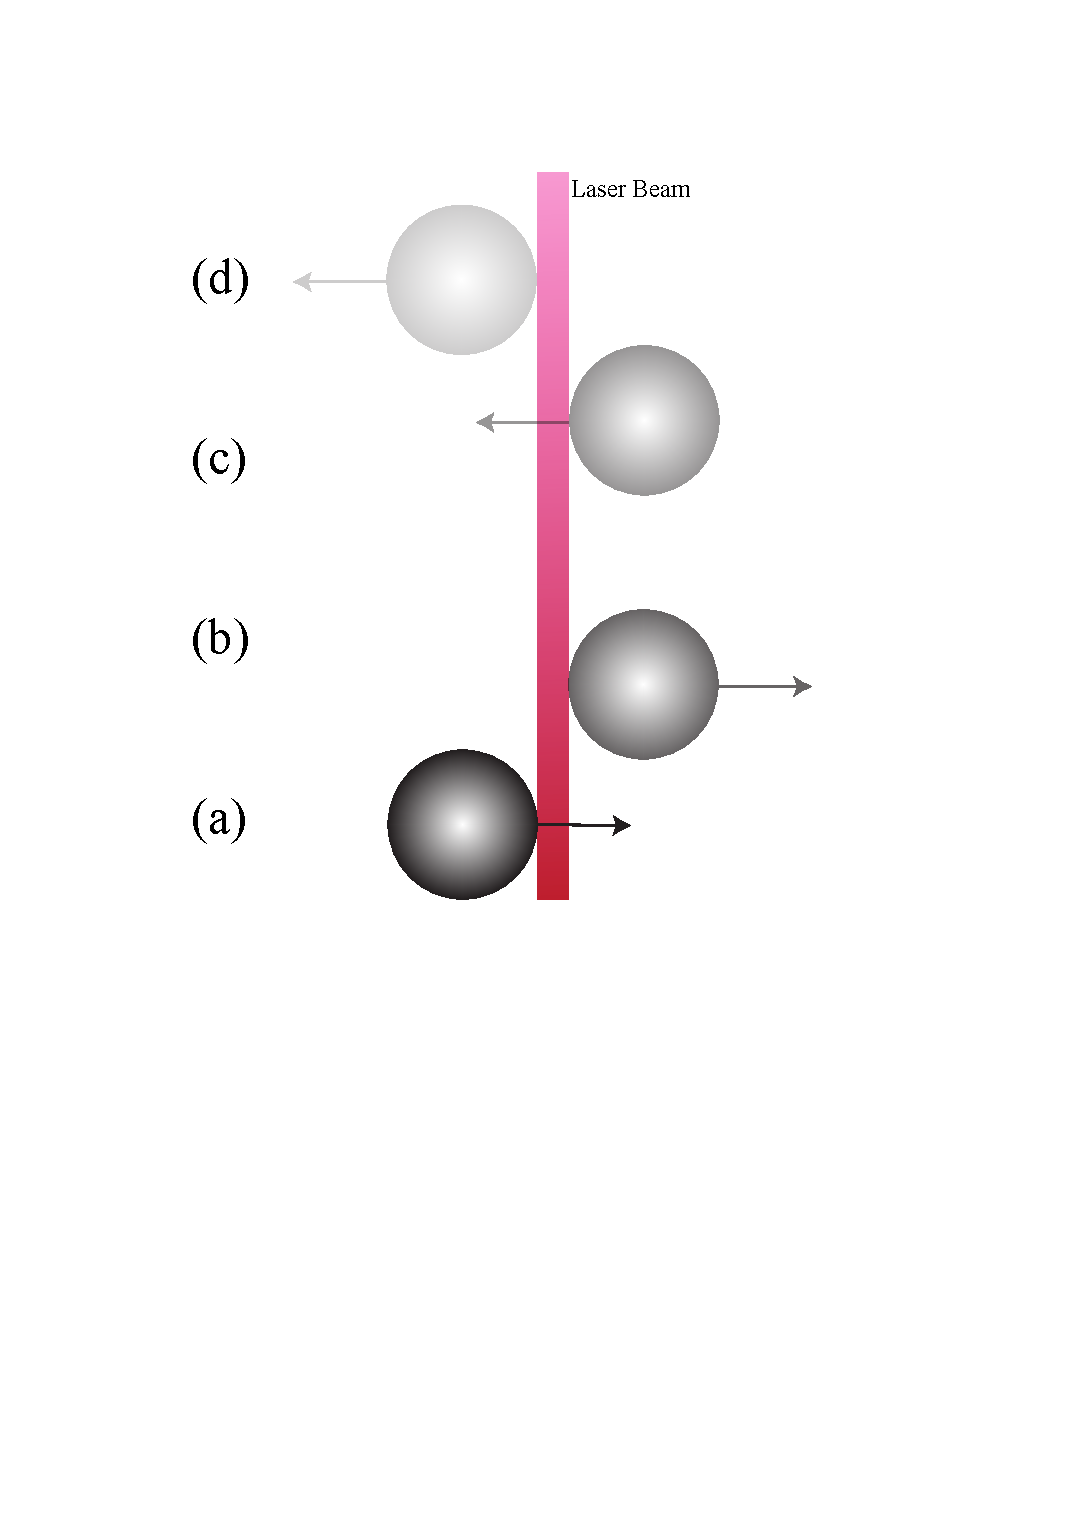
\includegraphics[width=.4\linewidth]{Figures/extractingData/OpticalSwitch.png}%
  \caption{The idea behind an optical switch---each time the pendulum enters or leaves the beam, a digital timing signal is recorded. In the figure, the pendulum is drawn a four different times; on the 5th crossing (not shown), one will have enough information to calculate the period.}
  \label{fig:opticalSwitch}%
\end{figure}

\begin{figure}[htb]\centering
 \includegraphics[width=0.85\linewidth]{Figures/extractingData/Output.png}%
  \caption{A plot (using Matplotlib) of the period vs time data from the full data set. Notice that Matplotlib automatically pulled out 3.462 s from the period axis on the left, so that the vertical ticks are spaced 0.4 ms apart, and over the course of 850 seconds, the period of the pendulum only changed by about 1 mS.}
  \label{fig:Output}%
\end{figure}


\textbf{Details for this Assignment }\\
\begin{enumerate}
	\item Read the file \href{http://media.usm.maine.edu/~pauln/dataFiles/periodData.txt}{periodData.txt}, and extract only lines with actual period values. Create an output file called {\textsf Filtered.dat} (which will go in your data folder---see Appendix~\ref{app:submission} for submission guidelines). 
	\item Plot this data from within your script using Matplotlib. I suggest you go to the Matplotlib gallery, find a simple x-y plot similar to what you want, and examine the code needed to create the plot.
	\item Once you create the plot on the screen, you can click the disk icon on the plot to save it to disk (in your \verb&LaTeX/Figures& folder) as a .png or a .pdf file. Alternatively, you can use the Matplotlib savefig() command to save a plot to disk (as usual, google for help on this).
	\item As a part two to this exercise, still using the data from periodData.txt (at \href{http://media.usm.maine.edu/~pauln/dataFiles/periodData.txt}{this link}) create a data file with all possible periods extracted; i.e. you can calculate the period as the difference in time between every 4th crossing:
	$$ \mathrm{Period}_i = t_{i+4} - t_i$$
In this scheme, you'll end up with roughly three times as many period measurements. Create a new output file called \textsf{tripleFiltered.dat}, and plot this data file as you did with \textsf{filtered.dat}. Keep in mind that you will have to modify your program to produce this data file. 
	\item Now write a short \LaTeX\ report about what you did. This is \textbf{not}
	a formal report, but simply an exercise to get your Linux/Python/LaTeX feet wet. When you're done, you'll have had experience with the three main tools we'll work with all semester, so the rest of the term will polish and deepen your familiarity with these tools.
	\item Don't forget to submit your completed assignment according to the format specified in Appendix~\ref{app:submission}. Your python scripts for part 1 and part 2 should of course be in your code folder.  
\end{enumerate}

\end{prob}

